\PassOptionsToPackage{unicode}{hyperref}
\PassOptionsToPackage{naturalnames}{hyperref}
\PassOptionsToPackage{table}{xcolor}

\documentclass[14pt]{beamer}

\mode<presentation> {

% The Beamer class comes with a number of default slide themes
% which change the colors and layouts of slides. Below this is a list
% of all the themes, uncomment each in turn to see what they look like.

%\usetheme{default}
%\usetheme{AnnArbor}
%\usetheme{Antibes}
%\usetheme{Bergen}
%\usetheme{Berkeley}
%\usetheme{Berlin}
%\usetheme{Boadilla}
%\usetheme{CambridgeUS}
%\usetheme{Copenhagen}
%\usetheme{Darmstadt}
%\usetheme{Dresden}
%\usetheme{Frankfurt}
%\usetheme{Goettingen}
%\usetheme{Hannover}
%\usetheme{Ilmenau}
%\usetheme{JuanLesPins}
%\usetheme{Luebeck}
%\usetheme{Madrid}
%\usetheme{Malmoe}
%\usetheme{Marburg}
%\usetheme{Montpellier}
%\usetheme{PaloAlto}
%\usetheme{Pittsburgh}
%\usetheme{Rochester}
%\usetheme{Singapore}
%\usetheme{Szeged}
%\usetheme{Warsaw}

% As well as themes, the Beamer class has a number of color themes
% for any slide theme. Uncomment each of these in turn to see how it
% changes the colors of your current slide theme.

%\usecolortheme{albatross}
%\usecolortheme{beaver}
%\usecolortheme{beetle}
%\usecolortheme{crane}
%\usecolortheme{dolphin}
%\usecolortheme{dove}
%\usecolortheme{fly}
%\usecolortheme{lily}
%\usecolortheme{orchid}
%\usecolortheme{rose}
%\usecolortheme{seagull}
%\usecolortheme{seahorse}
%\usecolortheme{whale}
%\usecolortheme{wolverine}

%\setbeamertemplate{footline} % To remove the footer line in all slides uncomment this line
%\setbeamertemplate{footline}[page number] % To replace the footer line in all slides with a simple slide count uncomment this line

\setbeamertemplate{navigation symbols}{} % To remove the navigation symbols from the bottom of all slides uncomment this line
\setbeamertemplate{frametitle continuation}[from second][(\insertcontinuationcountroman)]
}

\usepackage{graphicx} % Allows including images
\usepackage{booktabs} % Allows the use of \toprule, \midrule and \bottomrule in tables
% \usepackage[T1]{fontenc}
\usepackage[spanish]{babel}
\usepackage[utf8]{inputenc}
\usepackage{listings}
\usepackage{tikz}
\usetikzlibrary{calc,math,shapes.callouts,shapes.arrows,shapes.geometric,fit,positioning,arrows.meta}
\usetikzlibrary{positioning,backgrounds}
\usetikzlibrary{decorations.pathmorphing,math}
%\usepackage{iwona}
%\usepackage{marvosym}
%\usepackage{cfr-lm}
%\usepackage{pifont}
%\usepackage{keystroke}
%\usepackage{etoolbox}


\definecolor{mdwrojo}{HTML}{CC1A4C}
\setbeamercolor{titlelike}{fg=mdwrojo} % titulo
\setbeamercolor{frametitle}{fg=mdwrojo} % titulo
\setbeamercolor{section in toc}{fg=mdwrojo} % titulo
\setbeamercolor{subsection in toc}{fg=mdwrojo} % titulo
% https://tex.stackexchange.com/questions/185742/i-need-to-change-color-of-beamer-itemize-and-subitem-separately
%\setbeamercolor{itemize item}{fg=mdwrojo}
\setbeamercolor{itemize subitem}{fg=mdwrojo}
\setbeamercolor{block title}{bg=mdwrojo,fg=white}
\setbeamercolor{block body}{bg=mdwrojo!20}

%\setbeamercolor{block title}{bg=blue!30,fg=black}
%\setbeamercolor{block body}{bg=blue!20,fg=black}
%\setbeamercolor{block title alerted}{bg=red!30,fg=black}
%\setbeamercolor{block body alerted}{bg=red!20,fg=black}

\newcommand*{\murciabullet}{\kern1em
\includegraphics[height=1em]{img/mdw-bullet}}
\setbeamertemplate{itemize item}{\murciabullet}


% Language Definitions for CYPHER
\lstdefinelanguage{cypher}{
morecomment=[l][\color{gray}]{//},
morestring=[b][\color{olive}]\",
morestring=[b][\color{olive}]\',
morekeywords={MATCH,WHERE,LIMIT,CREATE,RETURN,DISTINCT,DELETE,DETACH,UNIQUE,MERGE,INDEX,ON,SET,LOAD,CSV,FOREACH,IN},
sensitive=true
}

%
% Listados de código
%
\lstset{%
basicstyle=\ttfamily\footnotesize,
commentstyle=\color{gray}\itshape\ttfamily,
keywordstyle=\color{blue!80}\bfseries\ttfamily,
stringstyle = \color{gray},
showstringspaces=false,
frame=tblr, % single, tb, ltrb % boxed listings, en mayusculas = doble linea
framerule=0pt,
tabsize=4, % tabulador = 2 espacios
captionpos=b,
backgroundcolor=\color{mdwrojo!20},
breaklines=true,
%backgroundcolor=\color{white},
%numbers=left, numberstyle=\tiny, stepnumber=2, numbersep=10pt,
xleftmargin=0.02\textwidth,
xrightmargin=0.02\textwidth,
language=java, % Por defecto
literate={«}{{\guillemotleft}}1
           {»}{{\guillemotright}}1
{á}{{\'a}}1 {é}{{\'e}}1 {í}{{\'i}}1 {ó}{{\'o}}1 {ú}{{\'u}}1
  {Á}{{\'A}}1 {É}{{\'E}}1 {Í}{{\'I}}1 {Ó}{{\'O}}1 {Ú}{{\'U}}1
  {à}{{\`a}}1 {è}{{\`e}}1 {ì}{{\`i}}1 {ò}{{\`o}}1 {ù}{{\`u}}1
  {À}{{\`A}}1 {È}{{\'E}}1 {Ì}{{\`I}}1 {Ò}{{\`O}}1 {Ù}{{\`U}}1
  {ä}{{\"a}}1 {ë}{{\"e}}1 {ï}{{\"i}}1 {ö}{{\"o}}1 {ü}{{\"u}}1
  {Ä}{{\"A}}1 {Ë}{{\"E}}1 {Ï}{{\"I}}1 {Ö}{{\"O}}1 {Ü}{{\"U}}1
  {â}{{\^a}}1 {ê}{{\^e}}1 {î}{{\^i}}1 {ô}{{\^o}}1 {û}{{\^u}}1
  {Â}{{\^A}}1 {Ê}{{\^E}}1 {Î}{{\^I}}1 {Ô}{{\^O}}1 {Û}{{\^U}}1
  {œ}{{\oe}}1 {Œ}{{\OE}}1 {æ}{{\ae}}1 {Æ}{{\AE}}1 {ß}{{\ss}}1
  {ű}{{\H{u}}}1 {Ű}{{\H{U}}}1 {ő}{{\H{o}}}1 {Ő}{{\H{O}}}1
  {ç}{{\c c}}1 {Ç}{{\c C}}1 {ø}{{\o}}1 {å}{{\r a}}1 {Å}{{\r A}}1
  {€}{{\euro}}1 {£}{{\pounds}}1
           {ñ}{{\~n}}1
           {Ñ}{{\~N}}1
           {¿}{{?`}}1
}

\colorlet{punct}{red!60!black}
\definecolor{background}{HTML}{EEEEEE}
\definecolor{delim}{RGB}{20,105,176}
\colorlet{numb}{magenta!60!black}

\lstdefinelanguage{json}{
    basicstyle=\ttfamily,
    stepnumber=1,
    numbersep=8pt,
    showstringspaces=false,
    breaklines=true,
%    frame=lines,
    moredelim=**[is][\color{red}]{@}{@},
    moredelim=**[is][\color{blue}]{º}{º},
%    backgroundcolor=\color{background},
    literate=
      {:}{{{\color{punct}{:}}}}{1}
      {,}{{{\color{punct}{,}}}}{1}
      {\{}{{{\color{delim}{\{}}}}{1}
      {\}}{{{\color{delim}{\}}}}}{1}
      {[}{{{\color{delim}{[}}}}{1}
      {]}{{{\color{delim}{]}}}}{1}
}

\definecolor{darkgray}{rgb}{.4,.4,.4}
\definecolor{purple}{rgb}{0.65, 0.12, 0.82}

\lstdefinelanguage{JavaScript}
{
  basicstyle=\ttfamily,
  keywords={typeof,new,true,false,catch,function,return,null,catch,switch,var,if,in,while,do,else,case
,break},
ndkeywords={class, export, boolean, throw, implements, import, this},
ndkeywordstyle=\color{darkgray}\bfseries,
sensitive=false,
comment=[l]{//},
morecomment=[s]{/*}{*/},
morestring=[b]',
morestring=[b]"
}

%% Macros comunes
\newcommand{\hide}[1]{}
\newcommand{\ra}{{\color{mdwrojo} $\Rightarrow${}~{}}}

\usepackage{fontspec}
\defaultfontfeatures{Ligatures=TeX,Numbers=OldStyle}
% \setmainfont{Aller_Lt.ttf}[
% BoldFont = Aller_Rg.ttf,
% ItalicFont = Aller_LtIt.ttf,
% BoldItalicFont = Aller_It.ttf]
\setsansfont
  [Ligatures=TeX, % recommended
   UprightFont={* Light},
   ItalicFont={* Light Italic},
   BoldFont={*},
   BoldItalicFont={* Italic}]
   {Roboto}
   % {Open Sans}
% \setsansfont
%   [Ligatures=TeX, % recommended
%    UprightFont={* Regular},
%    ItalicFont={* Italic}]
%   {Fira Sans}
%\setmainfont{Open Sans}[BoldFont={* Bold}]
% \setmonofont[Ligatures = TeX,
% UprightFont={* Light},
%    ItalicFont={* Light Italic},
%    BoldFont={* Medium},
%    BoldItalicFont={* Medium Italic}]{Input Mono}

%\setmonofont{Input Mono}
\setmonofont%[Scale=1.1]
 % [Ligatures=TeX, % recommended
 %  UprightFont={* Regular},
 %  ItalicFont={* Italic},
 %  BoldFont={* Bold},
 %  BoldItalicFont={* Bold Italic}]
%{Fira Mono}
{Source Code Pro}

\newsavebox{\mysubpic}

\usebackgroundtemplate{
%\setbox{\mysubpic}{
  \sbox{\mysubpic}{%
    \begin{tikzpicture}[remember picture,line width=1em,mdwrojo!30] %sub-picture
      \foreach \s in {1,...,\value{framenumber}}{
        \tikzmath{
          int \shift;
          \shift = (\s * 2);
          if Mod(\s,5) > 0 then {
            { \draw[xshift=\shift em] (0,0) -- (0,5em); };
          } else {
            { \draw[xshift=\shift em] (-.5em,3em) -- (-9.5em,1em); };
          };
       }
      }
    \end{tikzpicture}% needed, otherwise anchors are wrong!
  }

  \begin{tikzpicture}[remember picture,overlay,line width=2em]
    %\node[opacity=0.3, at=(current page.south east),anchor=south east,inner sep=0pt] {
%    \includegraphics[height=\paperheight,width=\paperwidth]{image}};
    \coordinate[at=(current page.north west)] (ul);
    \coordinate[at=(current page.south west)] (sw);
    \coordinate[at=(current page.south east)] (lr);
%    \path (ul) -- (lr) node[opacity=0.3,midway,anchor=center]{\usebox{\mysubpic}};
    \path (sw) -- (lr) node[opacity=.7,pos=.99,anchor=south east,scale=.1]{\usebox{\mysubpic}};
  \end{tikzpicture}
}

\hypersetup{%
  pdftitle={Big Data desde un punto de vista tecnológico},%
  pdfauthor={Diego Sevilla Ruiz},
  pdfsubject={Big Data, MDW'18},
  pdfkeywords={big data, mdw18}
}


%----------------------------------------------------------------------------------------
%       TITLE PAGE
%----------------------------------------------------------------------------------------

\title{Big Data:\\Un punto de vista
  tecnológico\thanks{\url{https://github.com/dsevilla/murciadigitalweek18}}}
\subtitle{MDW, 2018}

\author{Diego Sevilla Ruiz}
\institute[UMU]
{
Dpto. de Ingeniería y Tecnología de Computadores\\
Facultad de Informática\\
Universidad de Murcia\\
\medskip
\href{mailto:dsevilla@um.es}{\texttt{dsevilla@um.es}}
}
\date{Junio de 2018}

\makeatletter
\patchcmd{\beamer@sectionintoc}{\vskip1.5em}{\vskip1em}{}{}
\makeatother

\begin{document}

%\def\insertsectionnumber{\arabic{section}}

% \AtBeginSection[]{

% \begin{frame}[plain]

%   \begin{centering}
%     \begin{beamercolorbox}[sep=10pt,center]{part title}
%       {\huge \bf \textcolor{white}{\insertsectionnumber.~\insertsection}}
%     \end{beamercolorbox}
%   \end{centering}

%   \end{frame}
% }

%\def\insertsubsectionnumber{\arabic{subsection}}

% \AtBeginSection[]{
%   \begin{frame}<beamer>
%     \frametitle{\insertsubsection}

%     \tableofcontents[currentsection]
%   \end{frame}
% }
% \AtBeginSubsection[]{
%   \begin{frame}<beamer>
%     \frametitle{\insertsubsection}

%     \tableofcontents[currentsection,currentsubsection]
%   \end{frame}
% }
{
  \usebackgroundtemplate{%
    \vbox to \paperheight{\vfil
\includegraphics[width=\paperwidth]{img/mdw}\vfil}}
\begin{frame}
\titlepage % Print the title page as the first slide
\end{frame}
}

\section{Introducción}

\begin{frame}
  \frametitle{Big Data}
  \framesubtitle{\url{https://twitter.com/jmibl/status/390768769259163648}.}
\centering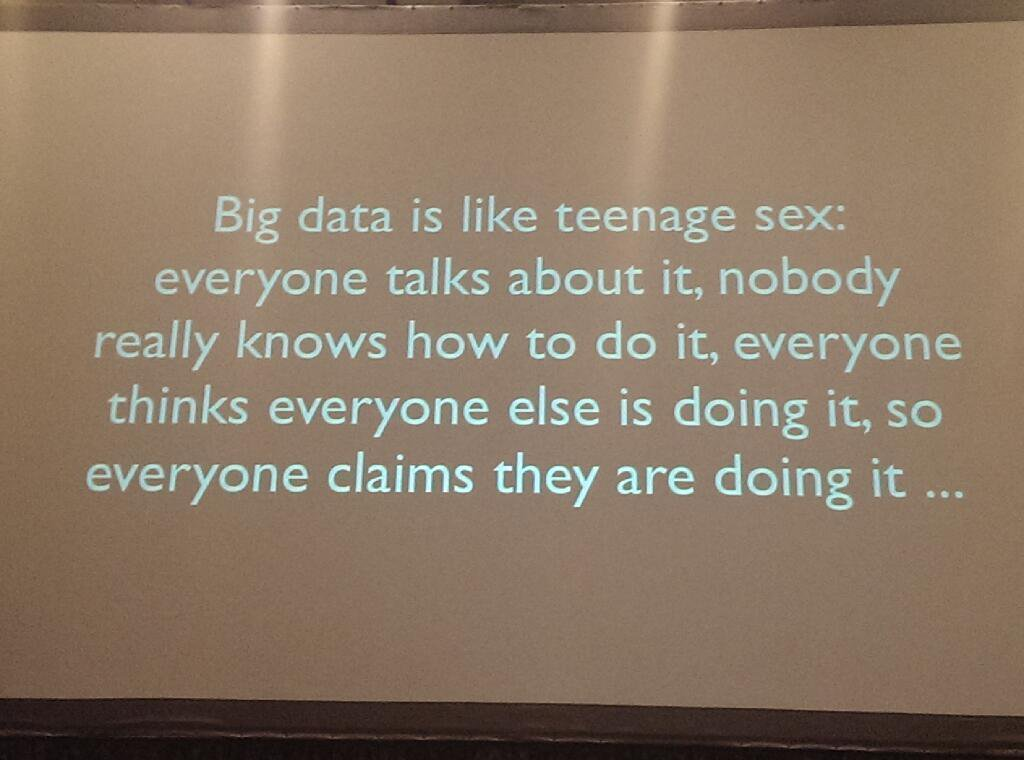
\includegraphics[width=.9\textwidth]{img/big_data_sex}
\end{frame}

\begin{frame}
  \frametitle{Big Data}
  \centering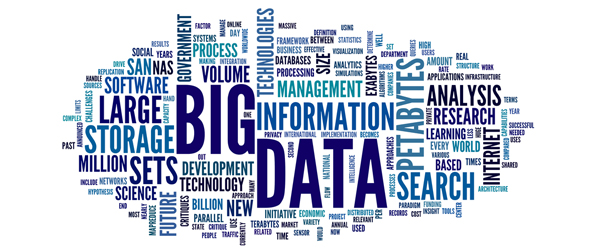
\includegraphics[width=\textwidth]{img/bigdata1}
\end{frame}

\begin{frame}
  \frametitle{Big Data -- 3Vs}
  \framesubtitle{\url{https://www.theviable.co/how-big-data-impact-to-corporate/3v-model-of-big-data/}}
\centering\includegraphics[width=\textwidth]{img/3v}
\end{frame}

\begin{frame}
  \frametitle{Big Data -- ¡¡¡8Vs!!!}
  \centering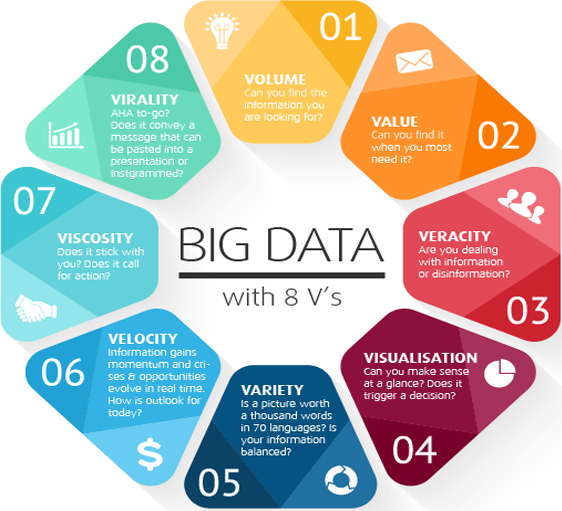
\includegraphics[width=.8\textwidth]{img/8V}
\end{frame}

\begin{frame}
  \frametitle{Big Data Landscape 2017}
  \framesubtitle{\url{http://mattturck.com/bigdata2017/}}
  \centering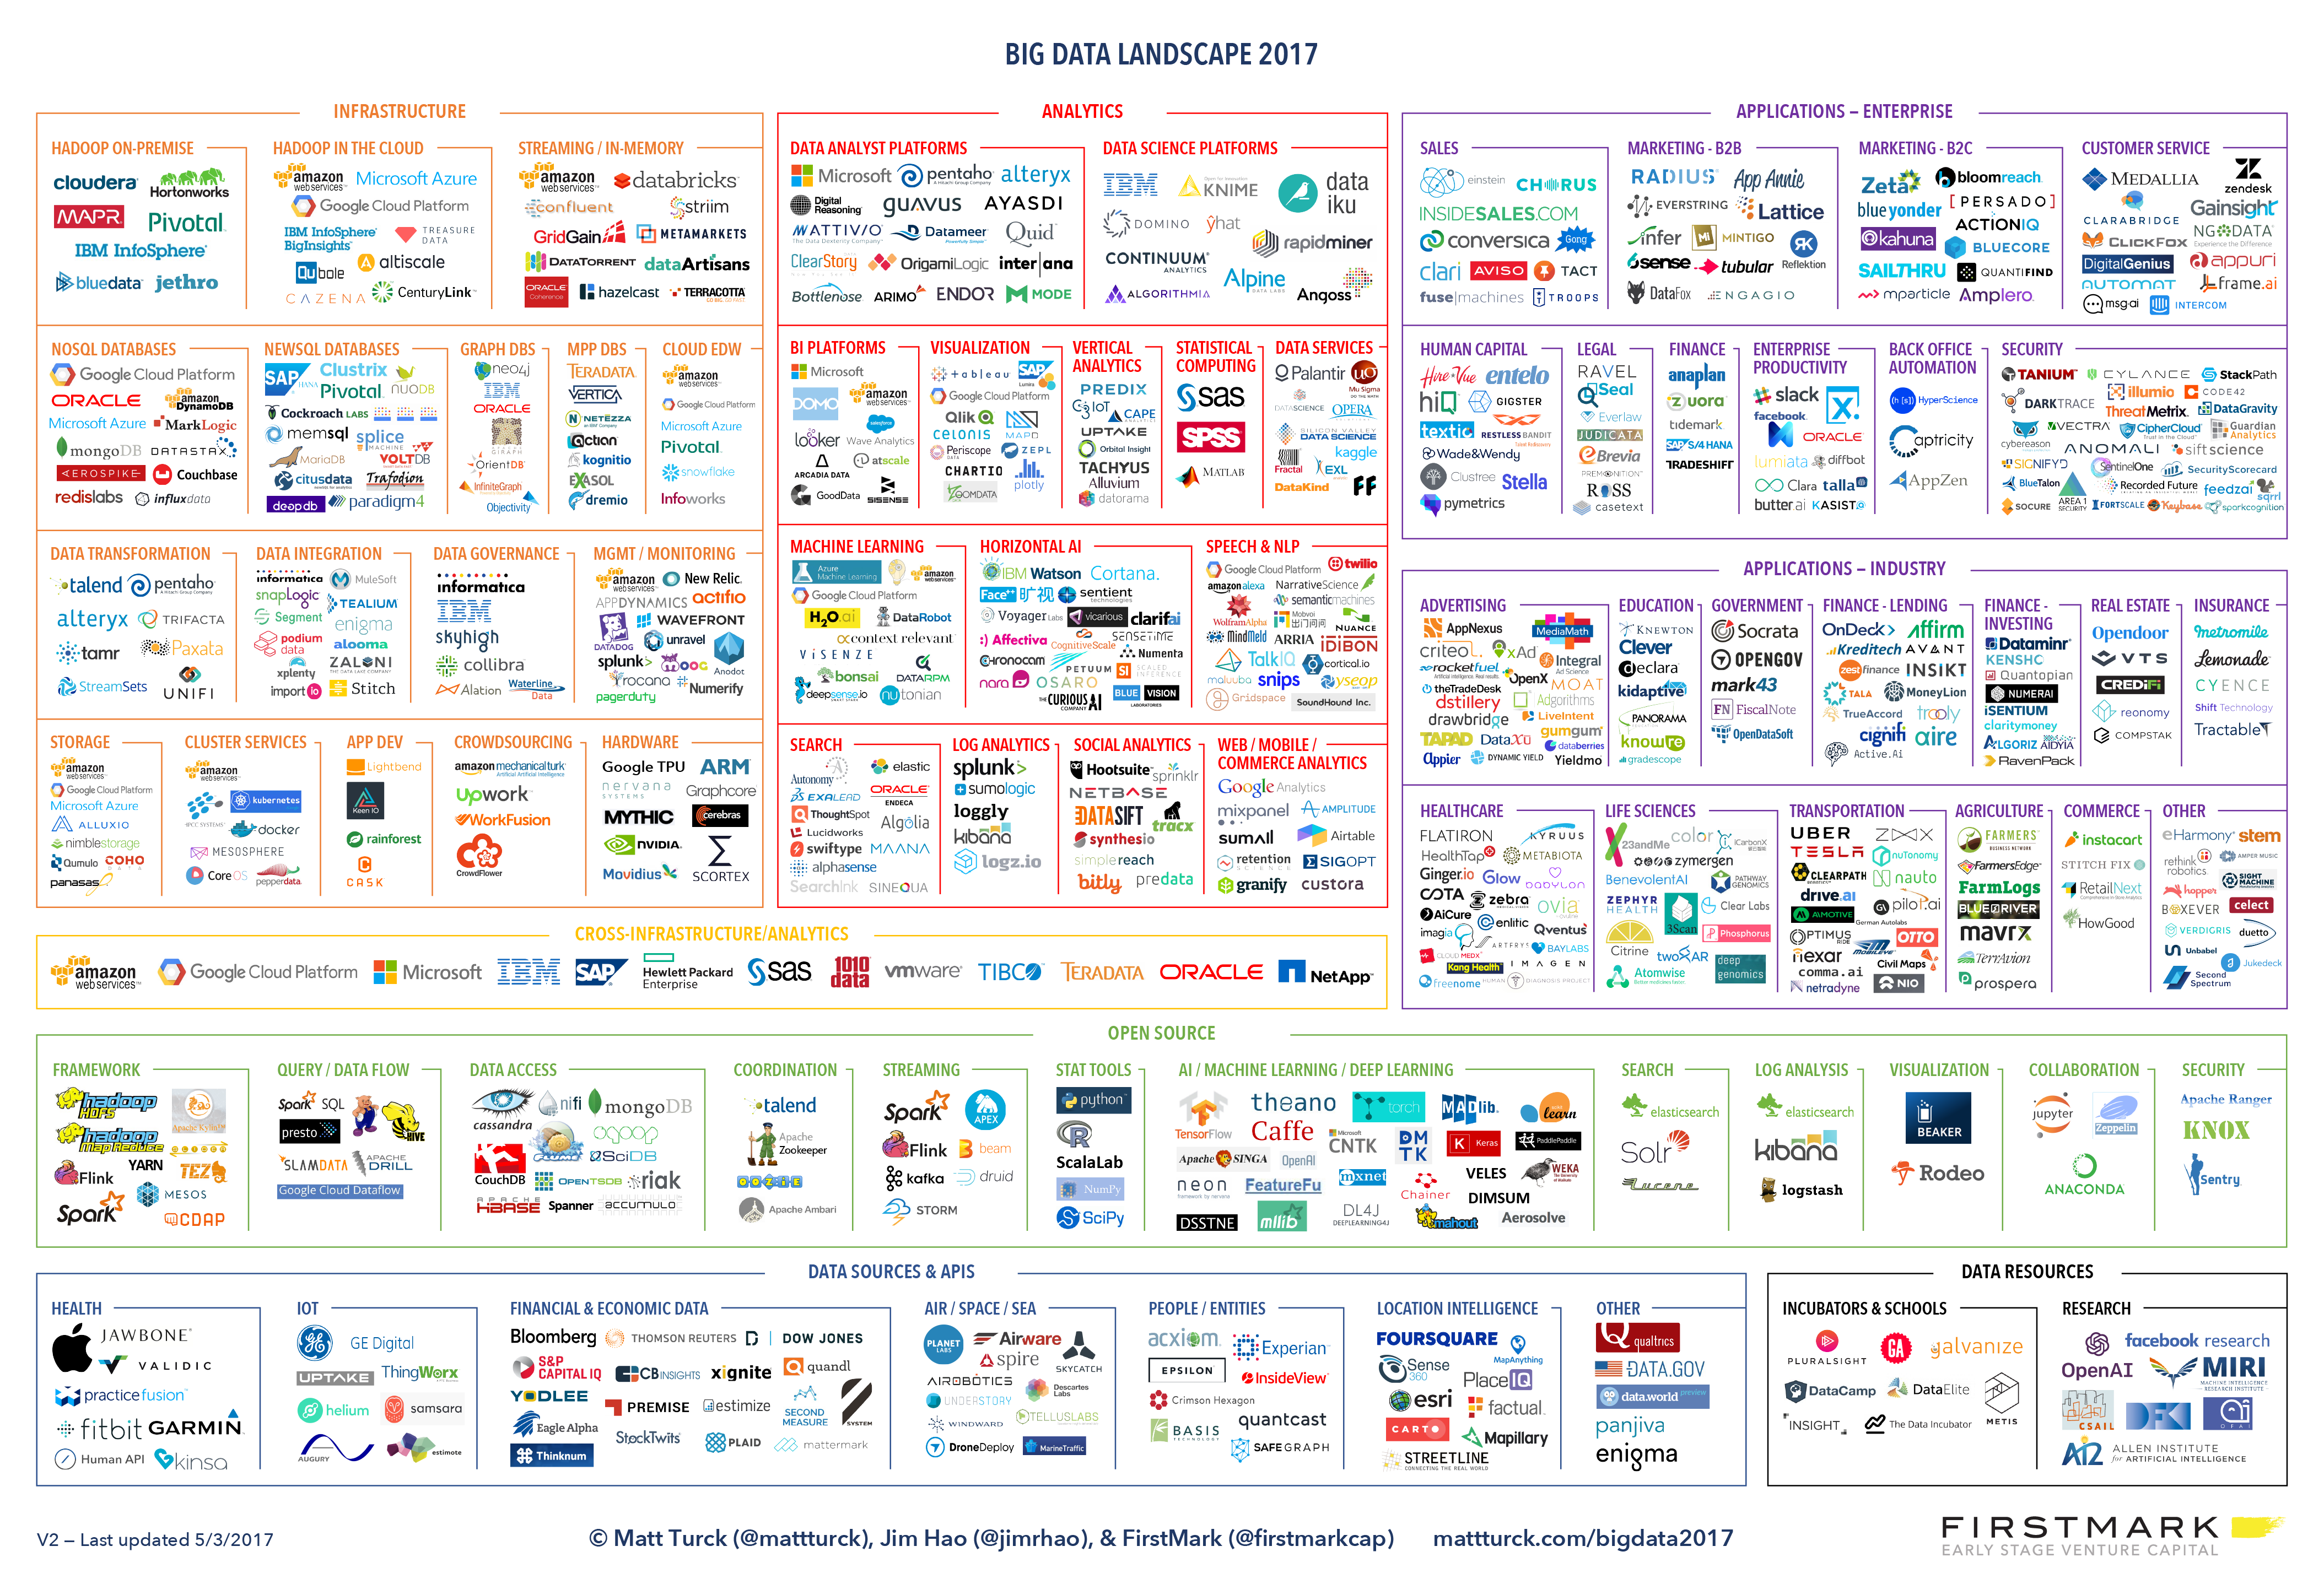
\includegraphics[width=\textwidth]{img/Big-Data-Landscape}
\end{frame}

\begin{frame}
  \frametitle{Big Data -- Un minuto del día}
  \framesubtitle{\url{https://www.domo.com/learn/data-never-sleeps-6}}
  \centering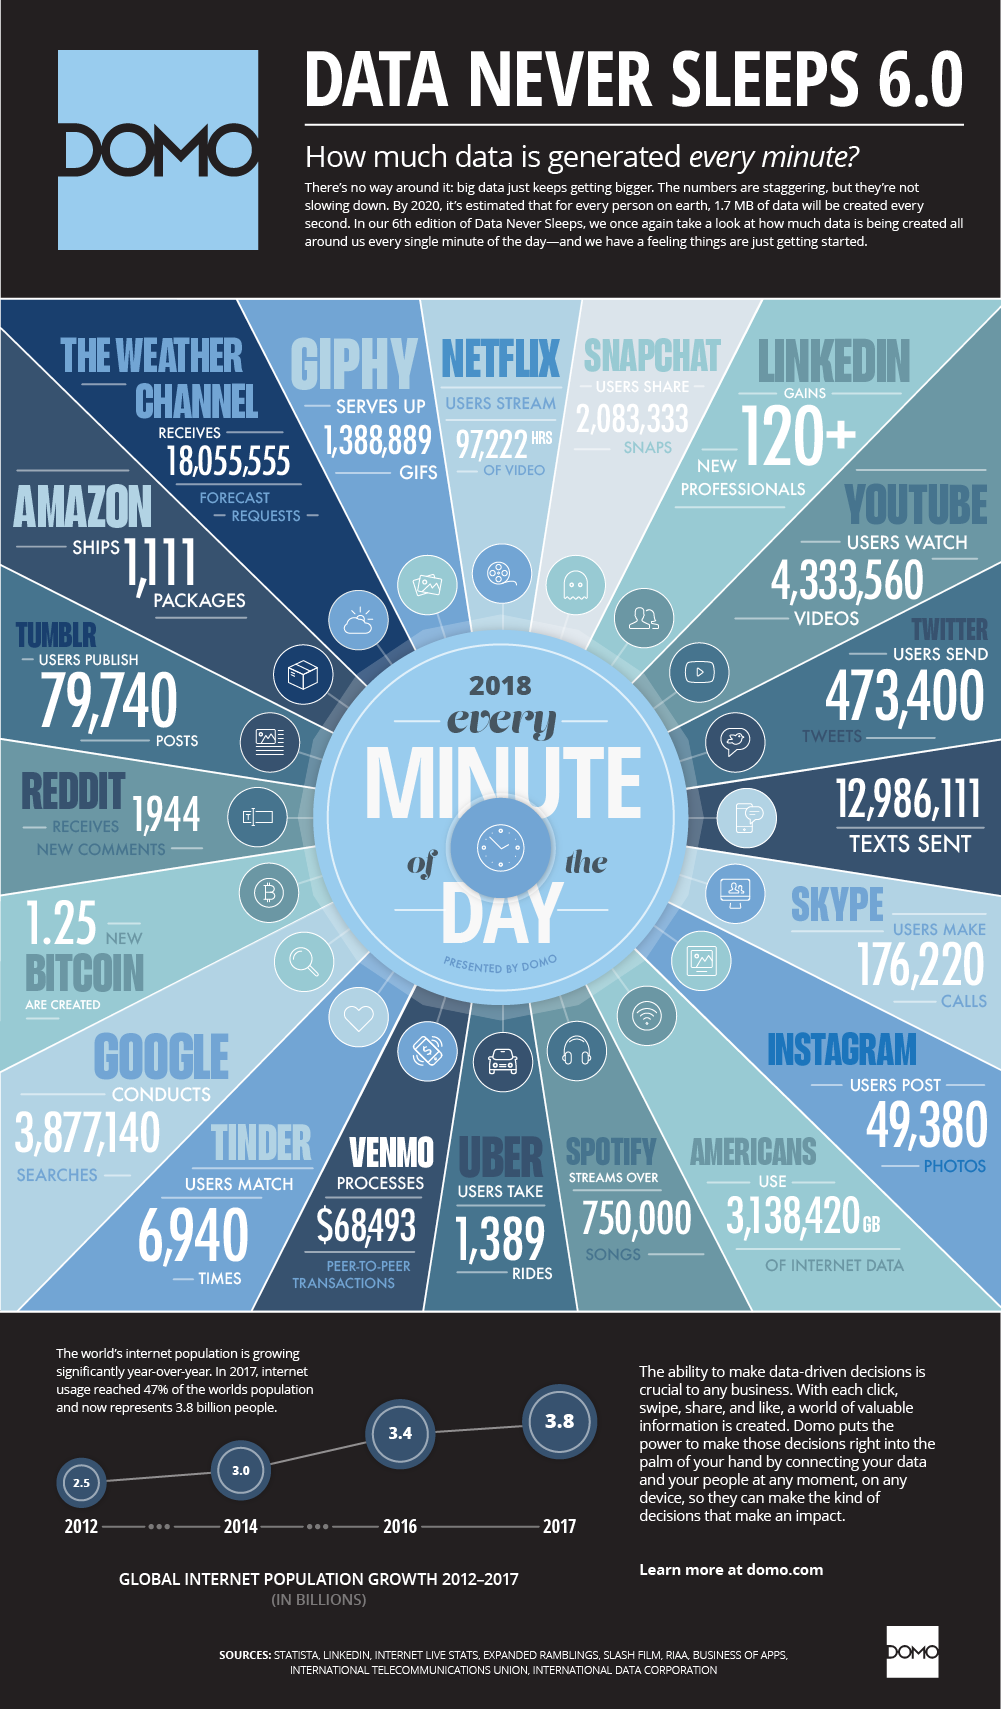
\includegraphics[height=.8\textheight]{img/data-never-sleeps-6}
\end{frame}

\begin{frame}
  \frametitle{Big Data -- Un minuto del día}
  \framesubtitle{\url{https://www.domo.com/learn/data-never-sleeps-6}}
  \centering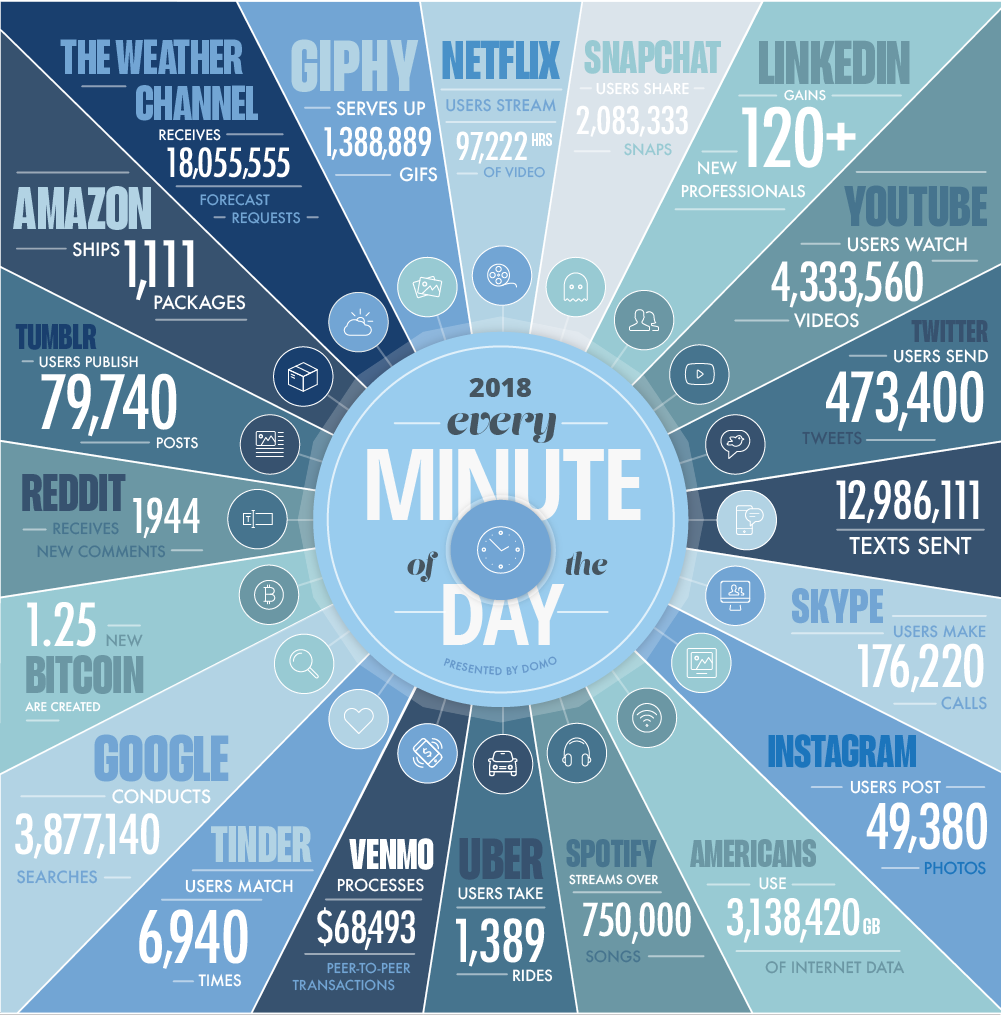
\includegraphics[height=.8\textheight]{img/data-never-sleeps-6-2}
\end{frame}

\begin{frame}
  \frametitle{Big Data -- ¡Y eso sin contar IoT!}
  \centering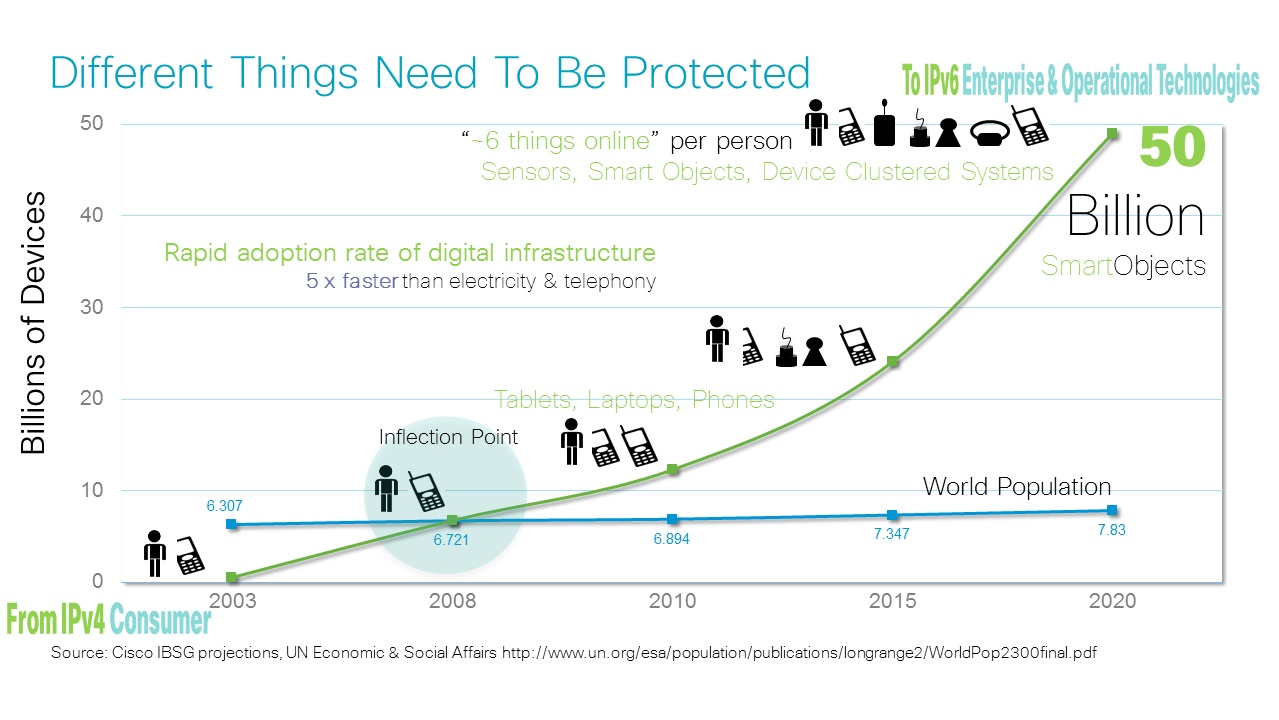
\includegraphics[width=\textwidth]{img/iot}
\end{frame}

\begin{frame}
  \frametitle{Big Data -- Airbus A350}
  \framesubtitle{\url{https://siliconsemiconductor.net/article/102842/Aviation_depends_on_sensors_and_big_data}}
  \centering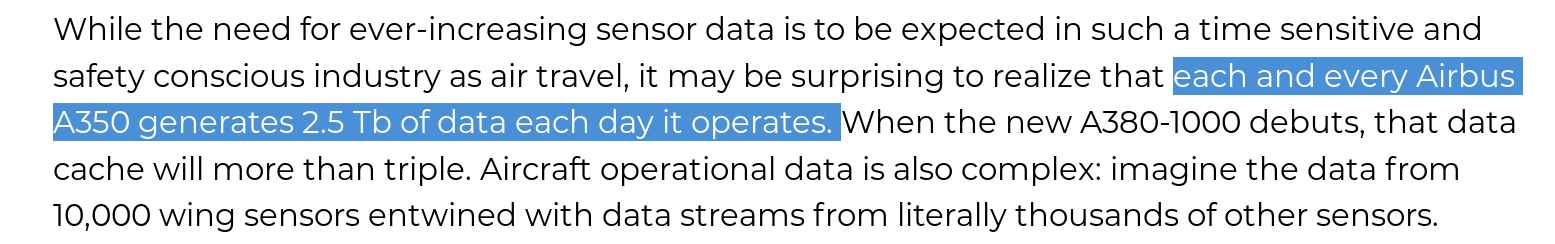
\includegraphics[width=\textwidth]{img/a350}
\end{frame}

\begin{frame}
  \frametitle{Big Data, entonces...}
  \begin{itemize}
  \item Recopilar todos los datos posibles
    \begin{itemize}
    \item Después serán útiles, se podrán analizar
    \item El coste de almacenamiento cada vez es menor
    \item Si no \ra{} coste de oportunidad
    \end{itemize}
  \item {\bfseries\itshape Data Science}
    \begin{itemize}
    \item El análisis ofrecerá {\bfseries\itshape conocimiento} para
      mejorar ({\bf valor})
    \end{itemize}
  \item Imposible procesar todo {\bfseries\itshape online}:
    \begin{itemize}
    \item Separación entre capa {\em batch\/} y capa {\em online}
    \item Lambda Architecture
    \end{itemize}
  \end{itemize}
\end{frame}

\begin{frame}
  \frametitle{Coste por GB}
  \centering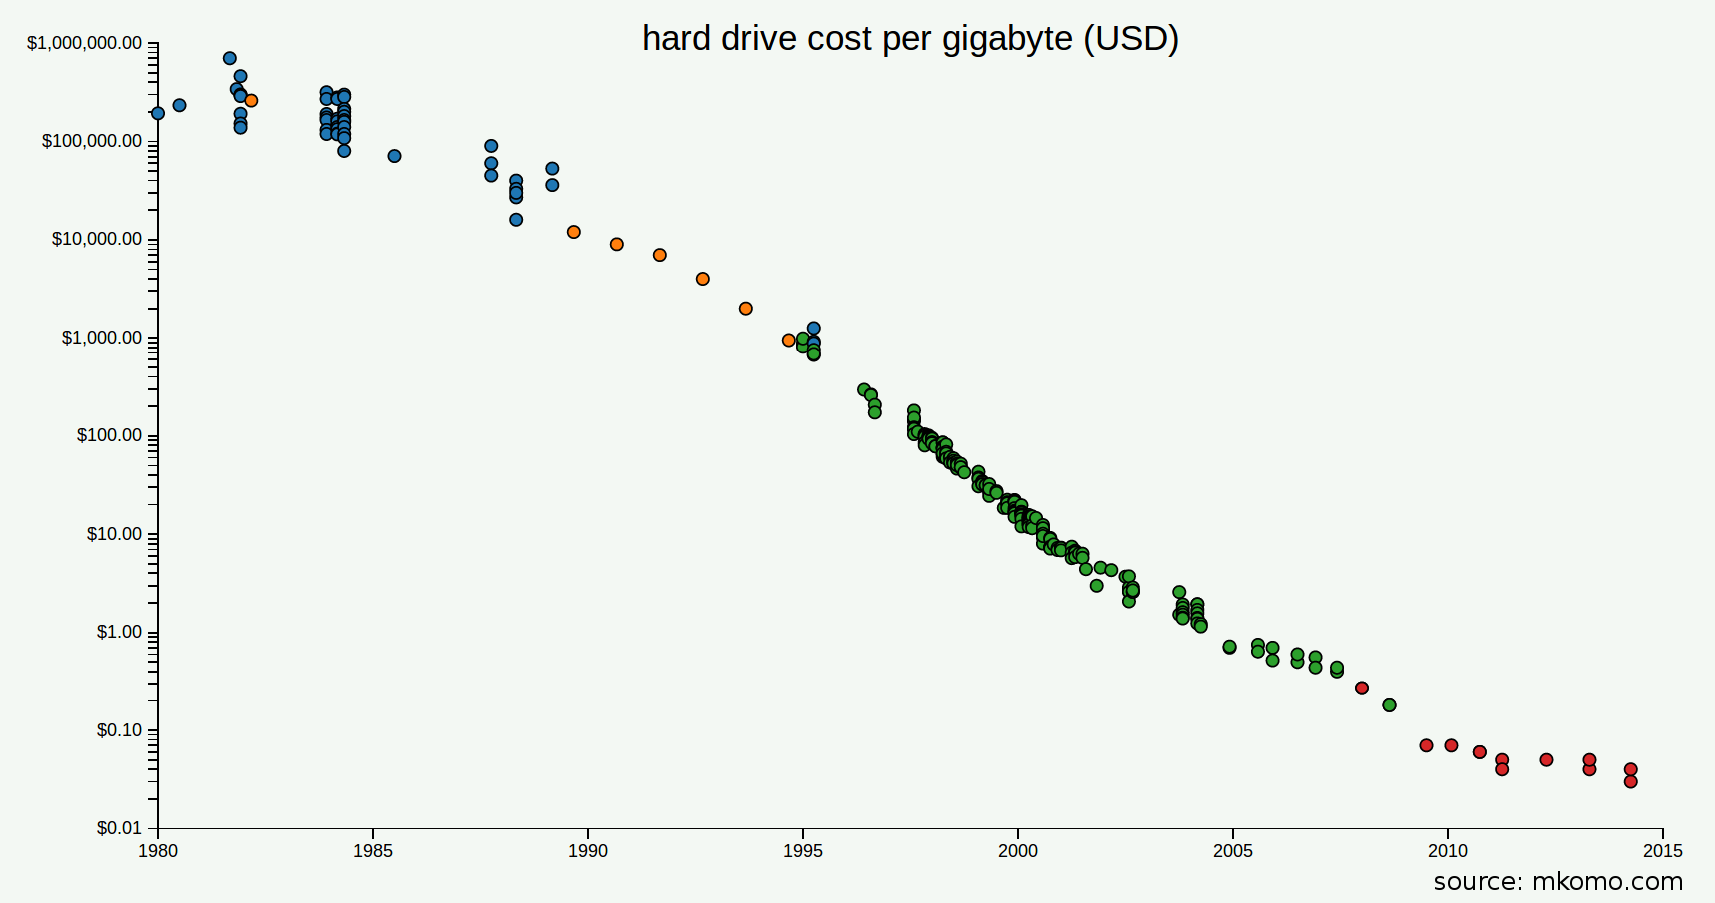
\includegraphics[width=\textwidth]{img/cost-per-gigabyte}
\end{frame}

\begin{frame}
  \frametitle{Lambda Architecture}
  \framesubtitle{\url{https://mapr.com/developercentral/lambda-architecture/}}
  \centering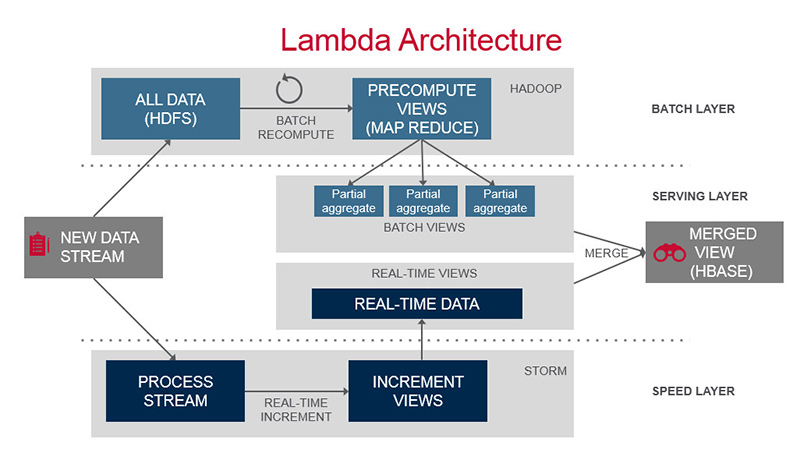
\includegraphics[width=\textwidth]{img/lambda-architecture}
\end{frame}

\section{Data Science}

\begin{frame}
  \frametitle{Data Science}
  \framesubtitle{Howe, 2013}
\vspace*{-.5em}
  \begin{quote}
    ``Next sexy job'' \\
    ``The ability to take data—to be able to understand it, to
process it, to extract value from it, to visualize it, to
communicate it—that’s going to be a hugely important skill.'' \\
  \hspace*\fill{\small--- Hal Varian, Google}
  \end{quote}
    \begin{quote}
``Data science is the civil engineering of data. Its acolytes
possess a practical knowledge of tools \& materials, coupled
with a theoretical understanding of what's possible.''\\
  \hspace*\fill{\small--- Mike Driscoll, Metamarkets}
  \end{quote}

\end{frame}

\begin{frame}
  \frametitle{Data Science}
  \framesubtitle{\url{http://drewconway.com/zia/2013/3/26/the-data-science-venn-diagram}}
\begin{center}
Drew Conway Venn Diagram of Big Data:
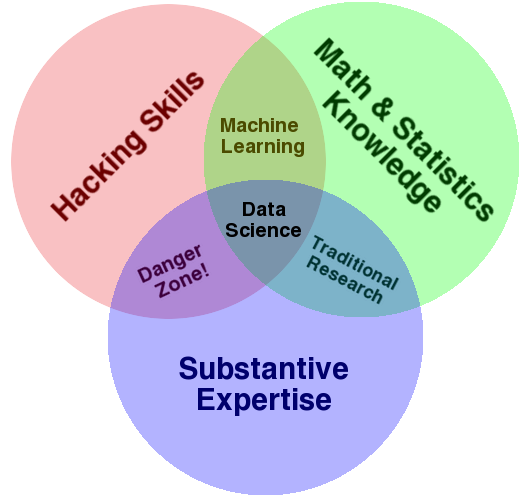
\includegraphics[width=.5\textwidth]{img/Data_Science_VD}
\end{center}
\end{frame}

\begin{frame}
  \frametitle{Data Science}

  Mike Driscoll’s three sexy skills of data geeks

  \begin{itemize}
  \item Statistics
    \begin{itemize}
    \item traditional analysis
\end{itemize}
\item Data Munging
  \begin{itemize}
  \item parsing, scraping, and formatting data
\end{itemize}
\item Visualization
  \begin{itemize}
  \item graphs, tools, etc.
\end{itemize}
\end{itemize}

\begin{block}{}
  \begin{center}
    (data wrangling, data jujitsu, data munging)
  \end{center}
\end{block}
\end{frame}

\begin{frame}[plain]
%  \frametitle{Data Science}
  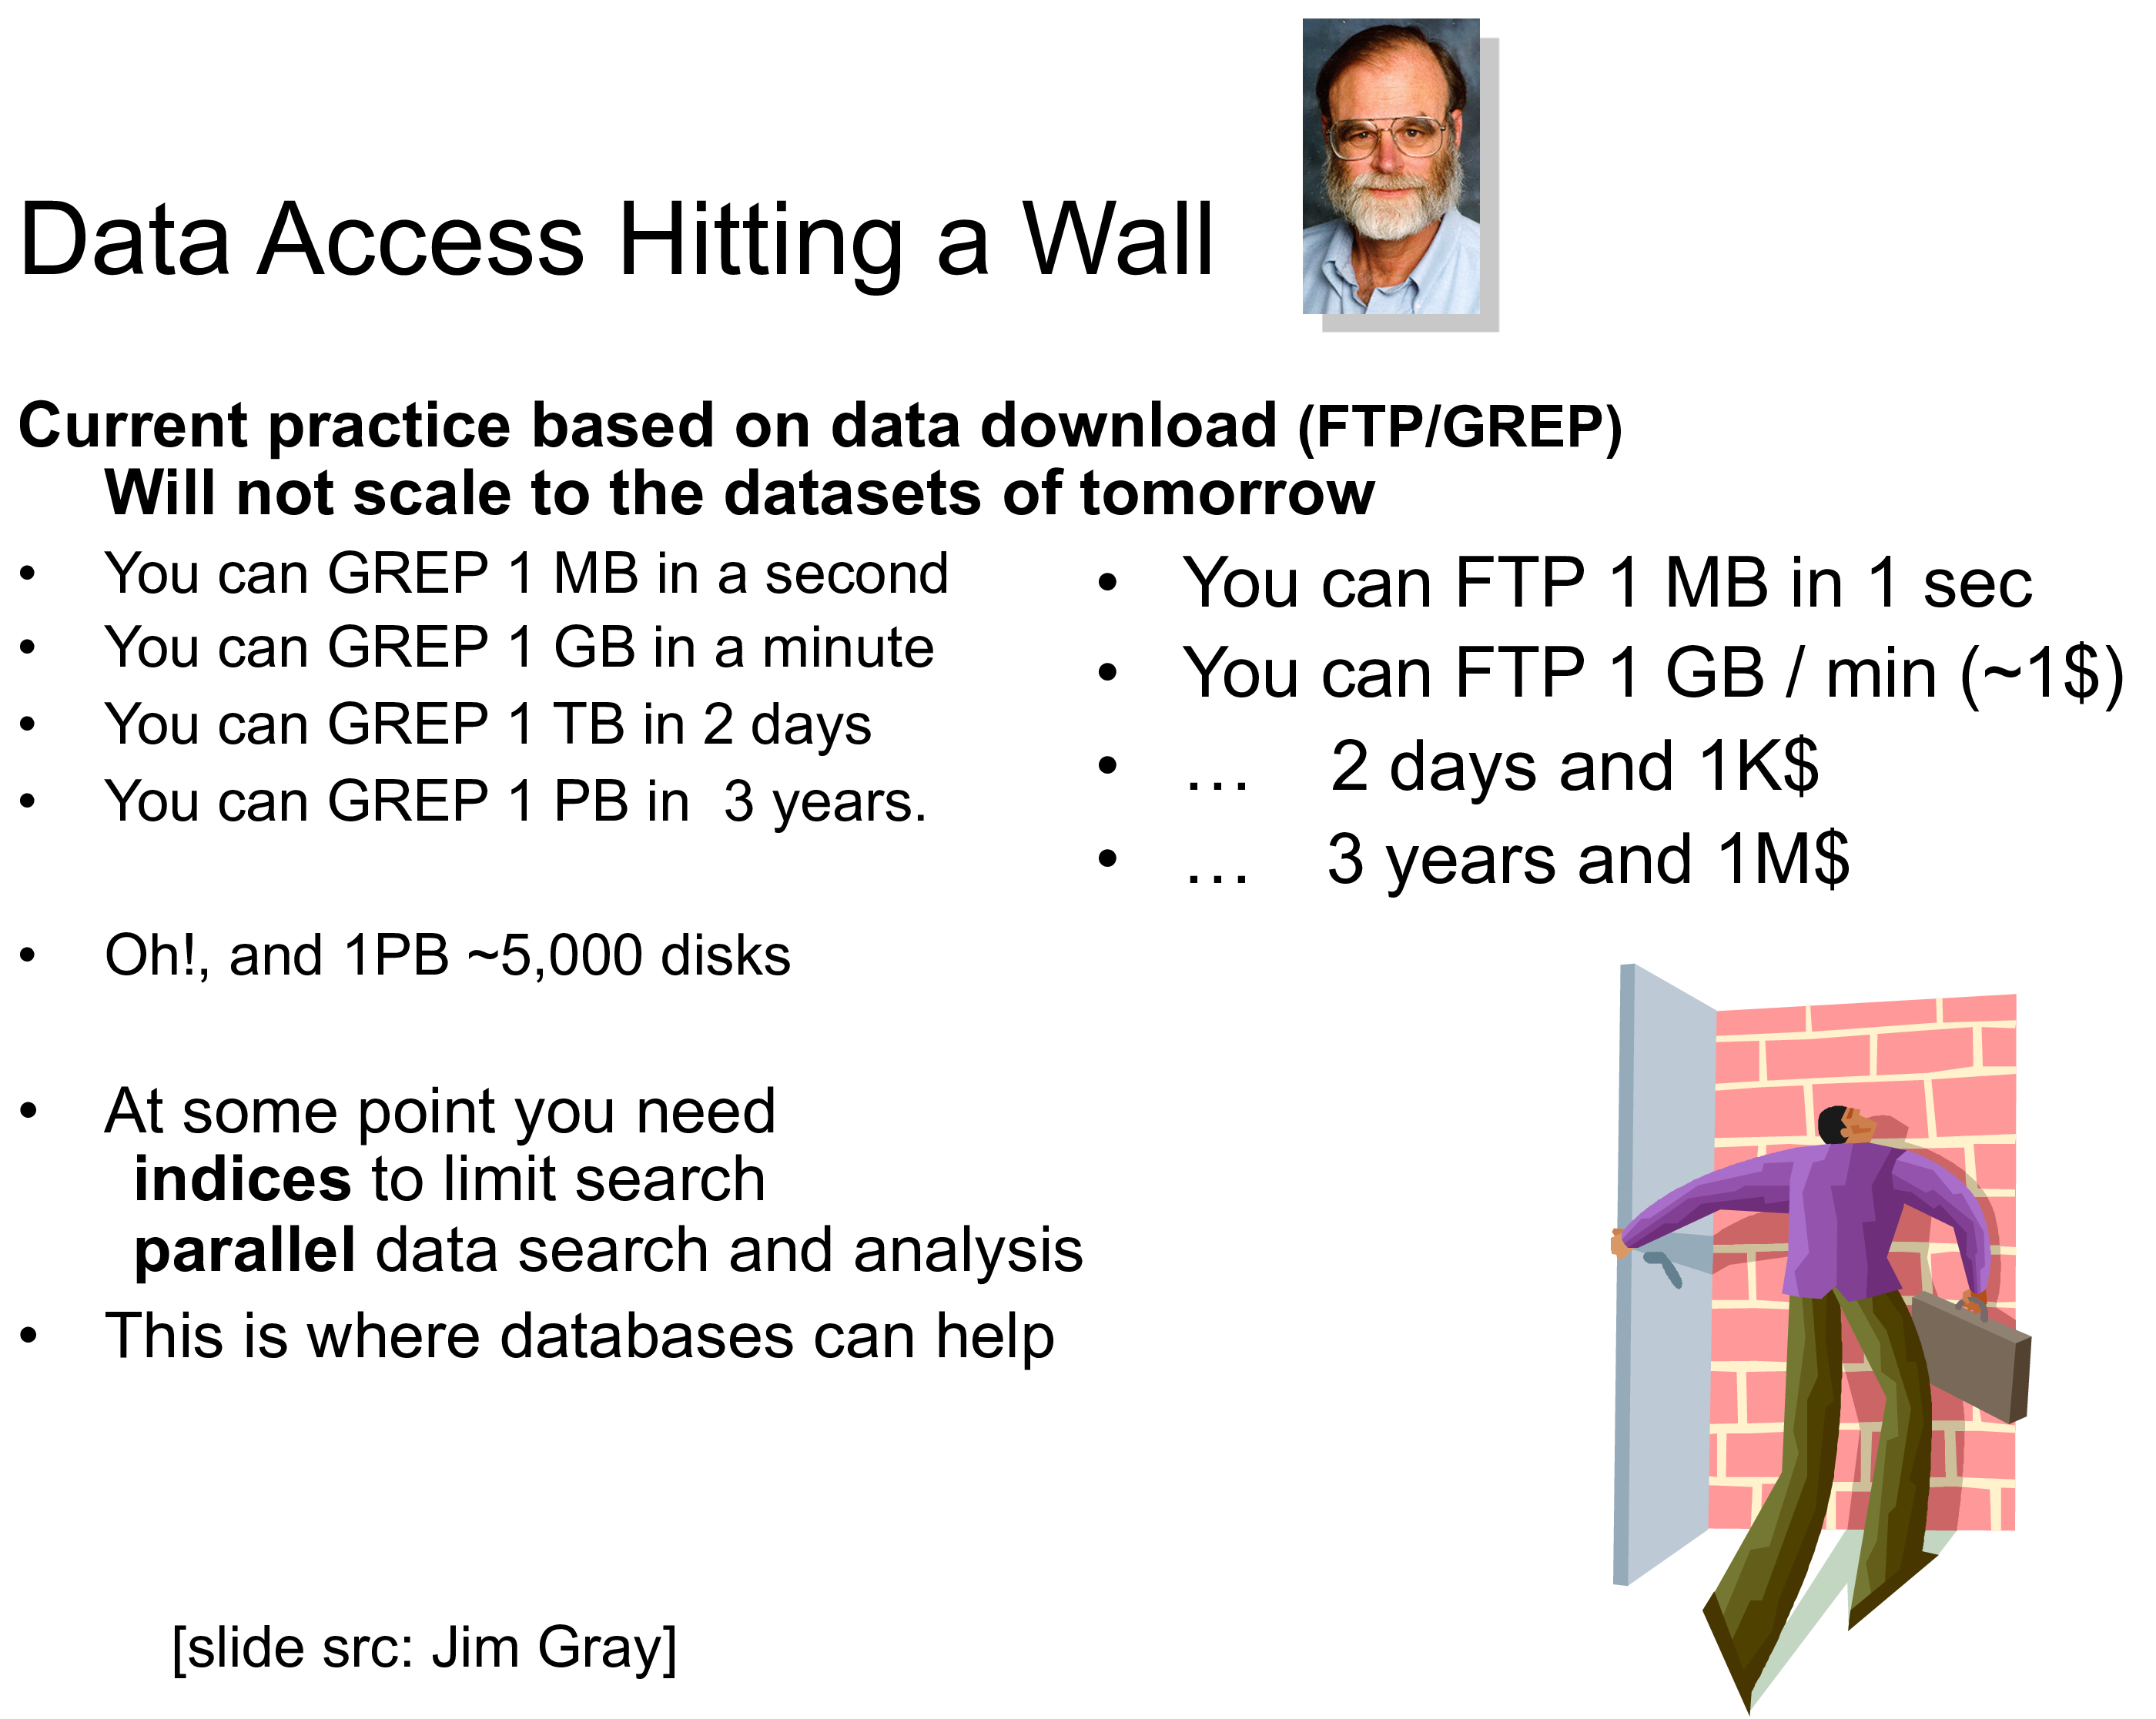
\includegraphics[width=\textwidth]{img/gray-grep}
\end{frame}


% [MUSIC] Welcome back. So I wanna talk a little bit about how the term
% Data Science relates to other fields of science. And, in particular, I
% wanna introduce this term, eScience, which to a first proximation you can
% think of is equivalent to Data Science. So while the term eScience is
% associated with astronomy and oceanography and biology, Data Science has
% been adopted more in business, but they involve a lot of the same
% concepts. So let me tell you about what's going on in science. So for
% thousands of years, scientific inquiry has been empirical, right? You
% observe the natural world, or in some cases maybe replicate the natural
% world, in a controlled environment in the laboratory and make
% observations about that. In the last few hundreds of years, science has
% accepted theoretical models as a valid method of inquiry, one that is
% reinforcing empirical methods. So, new theories suggest new experiments,
% and the theories help explain the observed data you get from the
% experiments. In the last 50 years or so, high speed computation has
% emitted an entirely new method of scientific inquiry. You can simulate in
% the computer phenomena that otherwise you can't observe directly and you
% can't reproduce in the lab. And even the theoretical models become too
% complex to solve analytically, using essentially paper and pencil, right?
% But you can actually start from initial conditions and run the simulation
% to get a result. So this is, maybe, the what goes on in the interior of
% stars, or the shift of tectonic plates, or the evolution of the universe,
% or the effects on the ecology from some species dying out, and so on. So
% that's fine, so that's three methods of inquiry. But in the last 10 years
% or so, there's been, arguably, a fourth method of scientific inquiry,
% which is to acquire massive data sets from instruments or from
% simulations, and then explore these data sets using new algorithms and
% new infrastructure. And so eScience is really about massive and complex
% data, data large enough to require automated or semi-automated analysis.
% You can't look at it, you can't inspect it directly. Okay. And so the
% relevant tools here are the same as those for data science, databases,
% visualization, scale out computing, maybe the NoSQL systems, machine
% learning techniques, web services, and so on. This idea of the fourth
% paradigm, there's a book that's in the reading list that you can refer to
% here. And there's some other articles in the reading list that you can
% also refer to. The story's been told lots of ways. The way I like to talk
% about this story is that science has always been about asking questions,
% but conventionally it was really about querying the world, right? You
% would sort of have data acquisition activities, experiments or field
% studies, that were coupled to very specific hypotheses, right? You had
% the question in mind, first, and went out and collected data. But
% eScience has really sort of shifted a bit where now you're downloading
% data en masse, you're downloading the world first, putting some sort of a
% representation into the computer and then querying that database to test
% your hypotheses. And so the data can be acquired independent of any
% specific hypothesis in some cases. Okay. And this is due in part to the
% cost of data acquisition dropping precipitously thanks to advances in
% technology, right, so the telescopes you can build now that we'll talk
% about in the next couple of slides can acquire enormous amounts of data
% at very high resolution. Okay. And in the life sciences you have sort of
% laboratory automation and you have high-throughput sequencing. In
% oceanography, the sensors are getting cheaper. The models, thanks to
% Moore's law and advances in computing, the simulations you can run are
% getting bigger and higher resolution and, therefore, producing larger and
% larger amounts of data, and so on. And so the rate at which data can be
% produced has far outpaced the rate that we can analyze it or come up with
% the questions we need to ask about it. Okay. The cost of finding,
% integrating and analyzing the data, and then communicating the results to
% others, is the new bottleneck. And this story should sound very similar
% to what we've been saying data science is all about.

\begin{frame}
  \frametitle{eScience, Data Science, 4º paradigma}
  \begin{itemize}
  \item Tradicionalmente, la ciencia se desarrollaba de forma {\bf
      empírica}, por observación, o reproduciendo condiciones en el
    laboratorio
  \item Desde hace unos cientos de años, los {\bf modelos teóricos} también
    se han aceptado como una forma de explicar sucesos, y sugerir nuevos
    experimentos
  \item En los últimos \~{}50~años, {\bf la simulación} se ha usado para
    reproducir condiciones especiales o no reproducibles. Modelos
    teóricos demasiado complejos para resolverlos analíticamente,
    parte de un estado inicial y comprueba a dónde se llega
  \end{itemize}
\end{frame}

\begin{frame}
  \frametitle{4º paradigma (ii)}
\vspace*{-.5em}
  \begin{itemize}
  \item Hoy: {\bf exploración basada en datos}
\begin{itemize}
\item Unifica teoría, experimentación y simulación
\item Los datos se capturan por instrumentos o bien se generan por
  simulaciones
\item Son procesados por software
  \item La información (y el conocimiento extraído) se almacenan en un
    ordenador
    \item Los científicos analizan los ficheros/bases de datos usando
     nuevas herramientas estadísticas y bases de datos capaces de
     gestionar cada vez más datos
   \item En vez de ``{\bf preguntar al mundo}'', se obtienen resultados de
     combinar conjuntos ``{\bf descargados}'' de datos de formas no
     previstas anteriormente
    \end{itemize}
\end{itemize}
\end{frame}

\begin{frame}
  \frametitle{The Fourth Paradigm}
  \framesubtitle{\url{https://twitter.com/aip_publishing/status/856825353645559808}}

  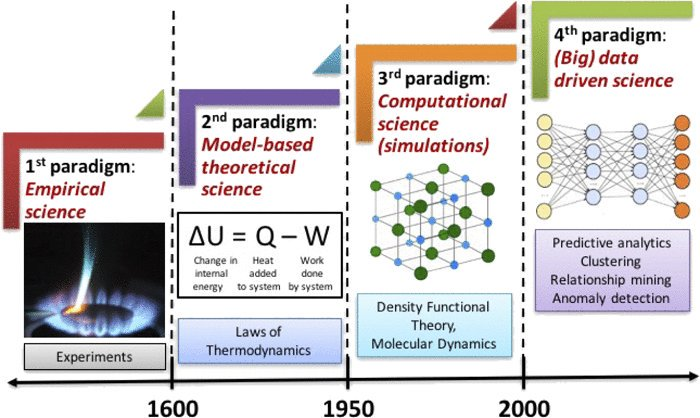
\includegraphics[width=\textwidth]{img/fourth-paradigm2}
\end{frame}

\begin{frame}
  \frametitle{The Fourth Paradigm}
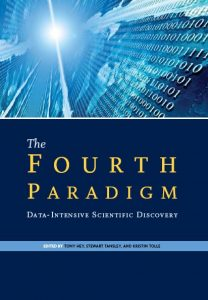
\includegraphics[height=12ex]{img/fourth-paradigm} {\bf Jim Gray}. {\em
    The Fourth Paradigm}, Microsoft Research,~2009
\end{frame}

\begin{frame}
  \frametitle{Huracán Sandy, 2012}
  \framesubtitle{\url{http://rpubs.com/JoFrhwld/sandy} (Howe, 2013)}
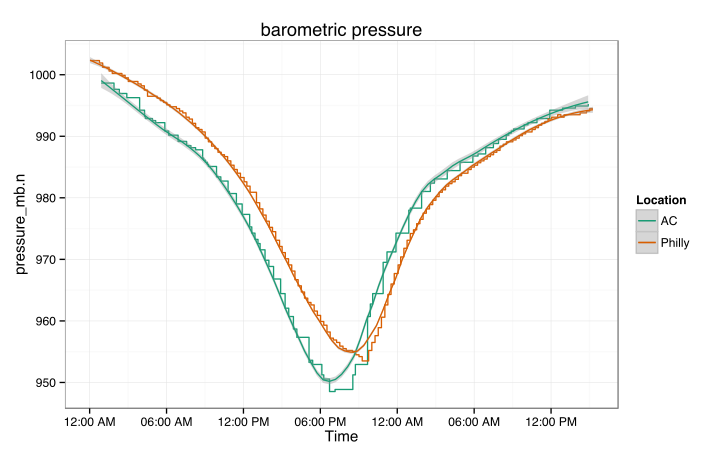
\includegraphics[width=\textwidth]{img/sandy}
\end{frame}

\begin{frame}
  \frametitle{¿Cuándo introdujo Apple el ``Swift''?}
  \framesubtitle{Una mirada al tag ``swift'' de todas las preguntas de
    Stackoverflow}
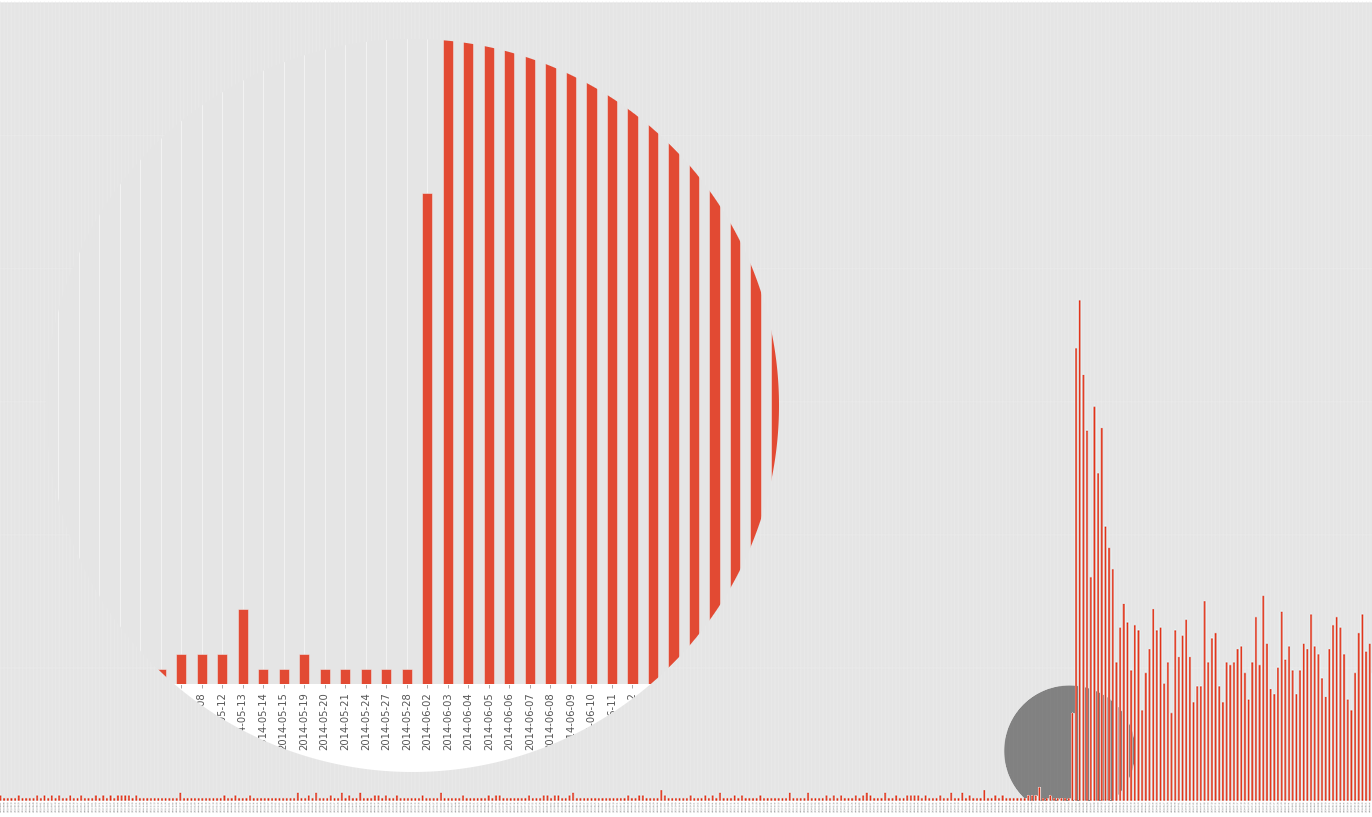
\includegraphics[width=\textwidth]{img/swift-tag}
\end{frame}

\section{Aplicación de Big Data a distintos ámbitos}

\begin{frame}
  \frametitle{Big Data -- Casos de éxito}
  \framesubtitle{Bernard Marr -- Big Data in Practice}
\centering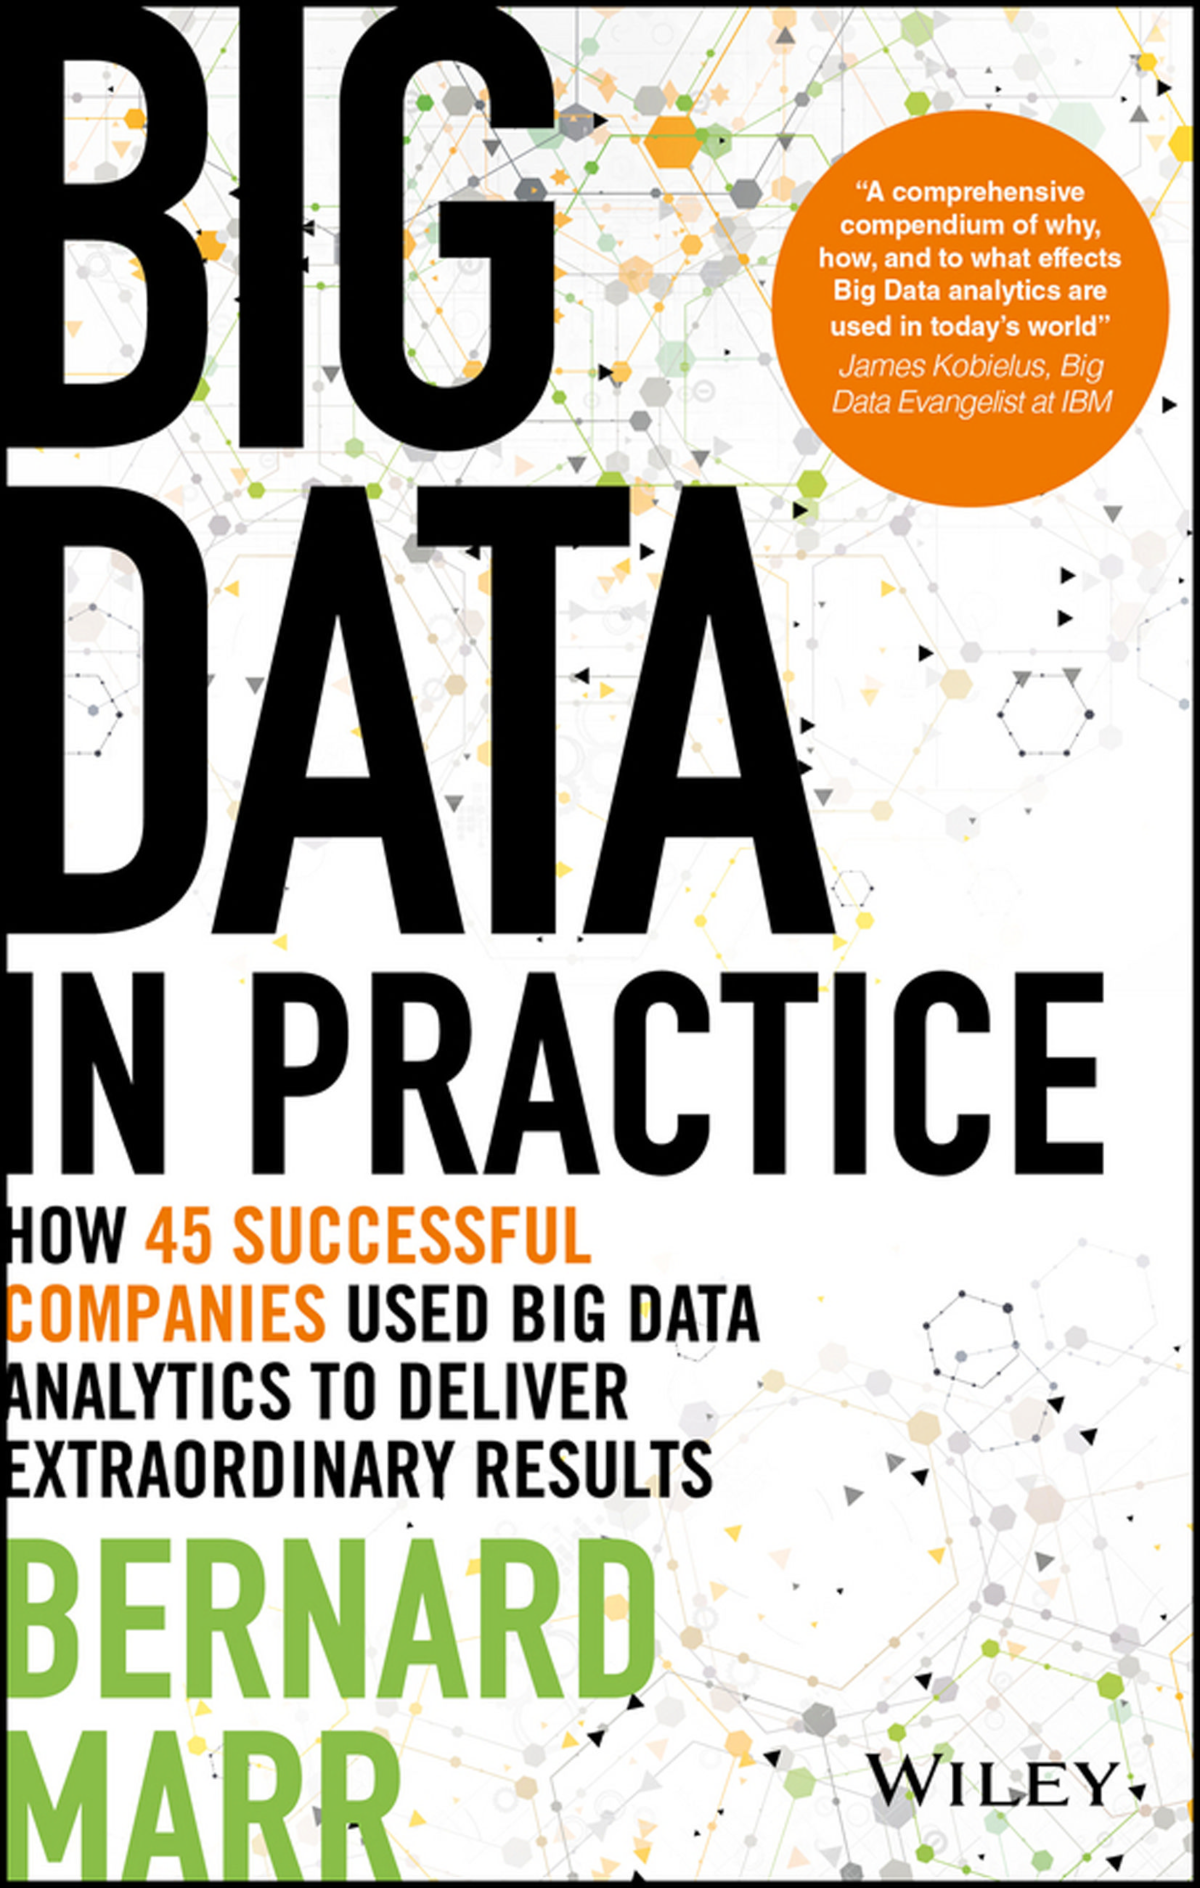
\includegraphics[height=.8\textheight]{img/marr-book}
\end{frame}

\begin{frame}[allowframebreaks]
  \frametitle{Big Data -- Caso de éxito: Walmart}
  \begin{itemize}
  \item Walmart tiene 20.000 tiendas en 28 países
  \item En 2015 se propusieron procesar 2,5~Petabytes de información cada
    hora
  \item Formó lo que denominó ``Data Café'', que procesaba la base de datos
    on-line de 40~Petabytes
  \item Redujeron tiempo de respuesta a problemas de semanas a {\bf 20
      minutos}
  \item Por ejemplo, detectaron que no se vendía un producto que sí se
    vendía en otras sucursales \ra{} Los empleados habían olvidado ponerlo
    en las estanterías
  \end{itemize}
\end{frame}

\begin{frame}[allowframebreaks]
  \frametitle{Big Data -- Caso de éxito: CERN}
\begin{itemize}
\item Sólo el {\em Large Hadron Collider} (LHC) genera 30~Petabytes al año
\item Los sensores del LHC detectan cientos de millones de colisiones de
  partículas
\item Hay que procesar esos datos para encontrar patrones de colisión para
  detectar partículas
\item 300~GB de datos por segundo \ra{} 300~MB/s filtrados
\end{itemize}
\end{frame}

\begin{frame}[allowframebreaks]
  \frametitle{Big Data -- Caso de éxito: Netflix}
\begin{itemize}
\item Inicialmente sólo tenía datos que asociaban un cliente, una película
  alquilada, la calificación y la fecha
\item Conforme se convirtió en {\em streaming}, pudo recopilar un conjunto
  mayor de datos
\item Añadió {\em tags\/} a cada película y episodio, lo que permitió
  generar contenido que, previsiblemente, iba a ser bien recibido
\item Oracle, después NoSQL y Cassandra
\item También utiliza tecnologías de Big Data como Hadoop, Pig y Hive (más
  después)
\end{itemize}
\end{frame}

\begin{frame}
  \frametitle{Big Data -- Casos de éxito}
  Y además: {\bf Rolls-Royce}, {\bf Shell}, {\bf Apixio}, {\bf Lotus F1
    Team}, {\bf Pendleton \& Son Butchers}, {\bf US Olympic Women’s Cycling
    Team}, {\bf ZSL}, {\bf Facebook}, {\bf John Deere}, {\bf Royal Bank of
    Scotland}, {\bf LinkedIn}, {\bf Microsoft}, {\bf Acxiom}, {\bf US
    Immigration And Customs}, {\bf Nest}, {\bf GE}, {\bf Etsy}, {\bf
    Narrative Science}, {\bf BBC}, {\bf Milton Keynes}, {\bf Palantir},
  {\bf Airbnb}, {\bf Sprint}, {\bf Dickey’s Barbecue Pit}, {\bf Caesars},
  {\bf Fitbit}, {\bf Ralph Lauren}, {\bf Zynga}, {\bf Autodesk}, {\bf Walt
    Disney Parks and Resorts}, {\bf Experian}, {\bf Transport for London},
  {\bf The US Government}, {\bf IBM Watson}, {\bf Google}, {\bf Terra
    Seismic}, {\bf Apple}, {\bf Twitter}, {\bf Uber}, {\bf Electronic
    Arts}, {\bf Kaggle}, {\bf Amazon}, etc.
\end{frame}


\begin{frame}[allowframebreaks]
  \frametitle{Big Data}
  \begin{itemize}
  \item Escalabilidad, concurrencia, distribución
  \item Map-Reduce
  \item Ecosistema Apache: Zookeeper, Hadoop, HBase, Spark, Hive, Impala
  \item Bases de datos NoSQL
  \item Arquitectura Lambda
  \end{itemize}
\end{frame}


\section{La importancia de la escalabilidad}

\pgfdeclareimage[height=2.7em]{sobremesa}{img/server1}%img/servidor}
\pgfdeclareimage[height=.7em]{switch}{img/switch1}%img/switch}

\newsavebox{\network}

\begin{lrbox}{\network}
\begin{tikzpicture}
  \foreach \x in {0,...,5}
    \foreach \y in {0,...,3}
    \node [] (\x\y) at (1.5*\x,1.5*\y) {\pgfuseimage{sobremesa}};

% switch
\node[inner sep=0pt] (switch) at (1.5*2.5, 1.5*4) {\pgfuseimage{switch}};

\begin{scope}[on background layer]
  \foreach \x in {0,...,5}
    \foreach \y in {0,...,3}
      \draw[gray!50] (switch)--(\x\y) ;
\end{scope}
\end{tikzpicture}
\end{lrbox}

\begin{frame}
\frametitle{Cambio de perspectiva: Red}

\begin{overlayarea}{\textwidth}{.8\textheight}
\only<1->{%
\begin{center}
\usebox{\network}
\end{center}%
}%
\only<2>{
\vspace*{-10em}
\begin{block}{Procesamiento distribuido}
\begin{itemize}
\item Necesidad de {\bf paralelización máxima}
\item {\bf Escalabilidad}
\item Explotación de la {\bf localidad de los datos}:
  \begin{itemize}
  \item Datos producidos en cada nodo se utilizan en siguientes iteraciones
  \item Cada nodo puede hacer de servidor para recibir datos
\end{itemize}
\end{itemize}
\end{block}
}%
\only<3>{
\vspace*{-9em}
\begin{block}{Procesamiento distribuido}
\begin{itemize}
\item Vuelta al modelo funcional inherentemente paralelo: (e.g. {\bf
    Map-Reduce})
\item Almacenamiento distribuido: (e.g. {\bf HDFS})
\item Coordinación distribuida: (e.g. {\bf Zookeeper})
\end{itemize}
\end{block}%
}%
\end{overlayarea}
\end{frame}


\begin{frame}[allowframebreaks,fragile]
\frametitle{Map-Reduce}

%  {\bf Map-Reduce} es el principal mecanismo de búsqueda y transformación en
%  BBDD NoSQL. Tiene su origen en {\bf lenguajes funcionales}:
%   \begin{block}{{\tt map()}}
%     Ejecuta una misma función sobre todos los elementos de un conjunto
%   \end{block}
%   \begin{block}{{\tt reduce()}}
%     Procesa un conjunto de valores para producir un valor de salida
%   \end{block}

% \framebreak

\begin{itemize}

\item Map-Reduce combina ambas operaciones:
\begin{itemize}
\item Una misma operación {\tt map()} a cada dato residente en un nodo se
  realiza de forma paralela en {\bf todos} los nodos simultáneamente
\item Con los resultados parciales de cada nodo, una función {\tt reduce()}
  genera un resultado (o un conjunto de resultados) final
\item Hay un proceso intermedio de {\em shuffle} para agrupar valores
  relacionados antes del {\tt reduce()}
\item Resultados parciales en el mismo nodo (localidad) $\Rightarrow$
  procesamientos {\bf en cadena}
\end{itemize}
\end{itemize}


\framebreak

\centering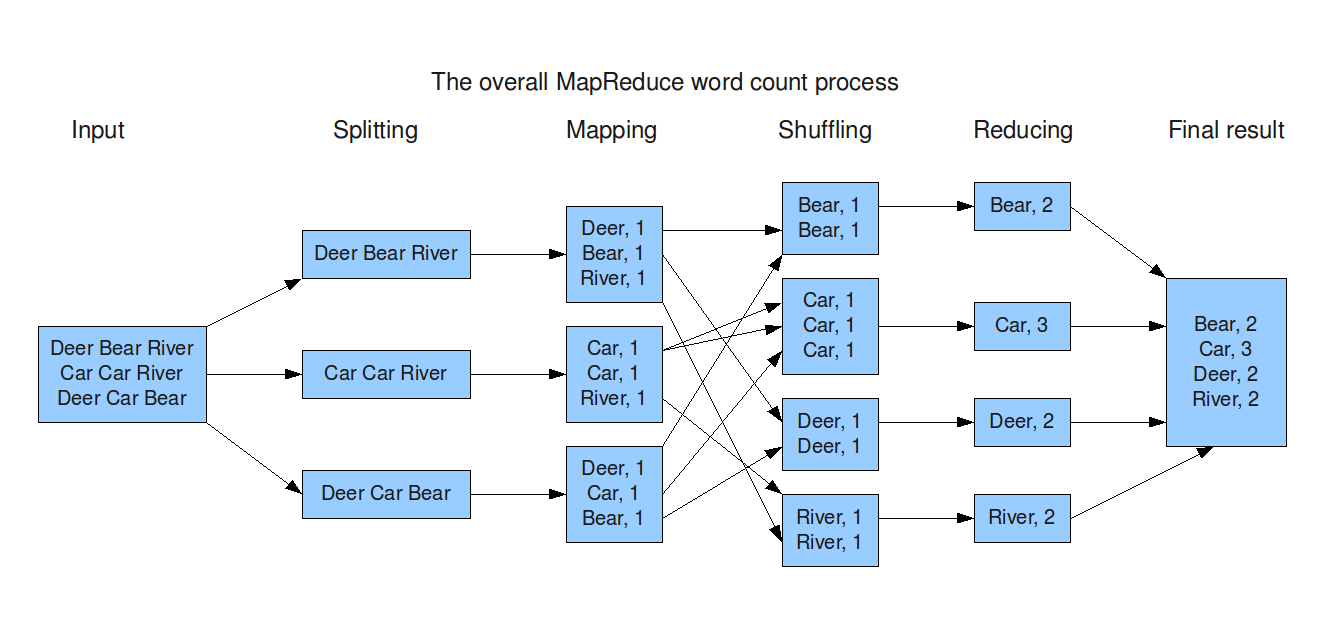
\includegraphics[width=\textwidth]{img/MapReduceWordcount}
(de \url{http://www.milanor.net/blog/an-example-of-mapreduce-with-rmr2/})
\end{frame}

\begin{frame}
\frametitle{Map-Reduce en entornos Big Data}
\begin{itemize}
  \item Entrada \ra{} siempre pares $<key,value>$

  \item {\tt map()} produce otro conjunto de valores
    $\{<key1,value1>,<key2,value2>,...\}$

\item {\em Shuffle} agrupa los valores con la misma clave:
\begin{displaymath}
\{<key1,\{val1,val3,...\}>,<key2,\{val2,val4,...\}>,...\}
\end{displaymath}

\item {\tt reduce()} procesa cada lista de valores con la misma clave, y
  produce otros elementos $<key',value'>$

\item Hay procesamientos difíciles de expresar en Map-Reduce $\Rightarrow$
  varias operaciones M/R {\bf en cadena}
  \end{itemize}

\end{frame}

\begin{frame}
  \frametitle{Hadoop}
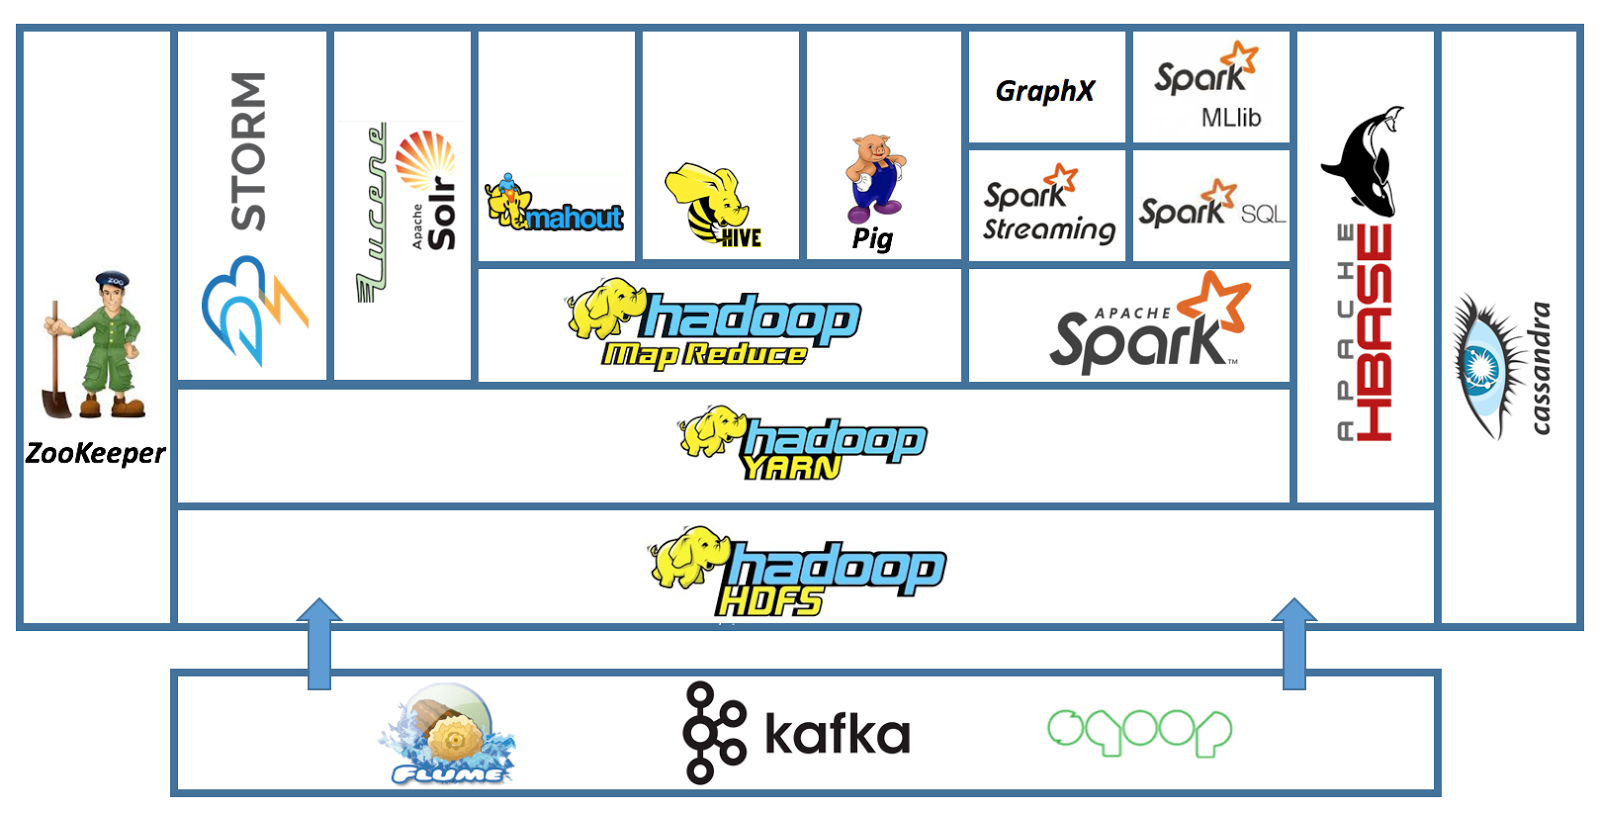
\includegraphics[width=\textwidth]{img/hadoop}
\end{frame}

\begin{frame}
  \frametitle{Hadoop -- YARN}
 \framesubtitle{\url{http://bigdataanalyticsnews.com/hadoop-yarn-adds-application-threads-big-data-users/}}
  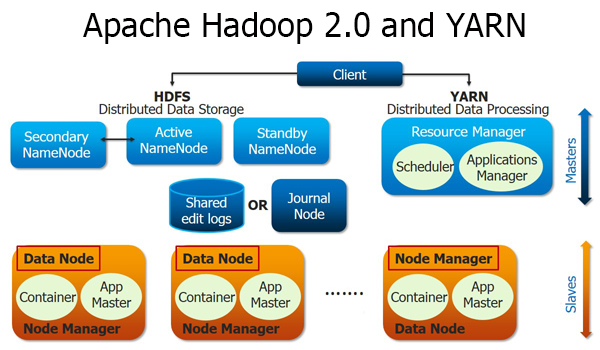
\includegraphics[width=\textwidth]{img/hadoop-yarn}
\end{frame}

\begin{frame}[allowframebreaks]
  \frametitle{HDFS}
HDFS posee una arquitectura distribuida:
    \begin{itemize}
    \item {\bf NameNode} -- Almacena información sobre qué partes
      ({\bfseries\itshape Chunks}) tiene cada fichero, y dónde están
      almacenadas (y replicadas)
    \item {\bf Secondary Namenode} -- Sustituto del {\bf NameNode} en caso
      de fallo
    \item {\bf DataNode}s -- Almacenan los {\em chunks\/} de cada fichero.
      Cada {\em chunk} puede estar replicado un número de veces,
      dependiendo de la configuración de HDFS
    \item {\bf Zookeeper} -- Se encarga de mantener una consistencia de
      {\em clúster} (saber qué nodos hay conectados y activos) y
      sincronización de datos
    \end{itemize}
  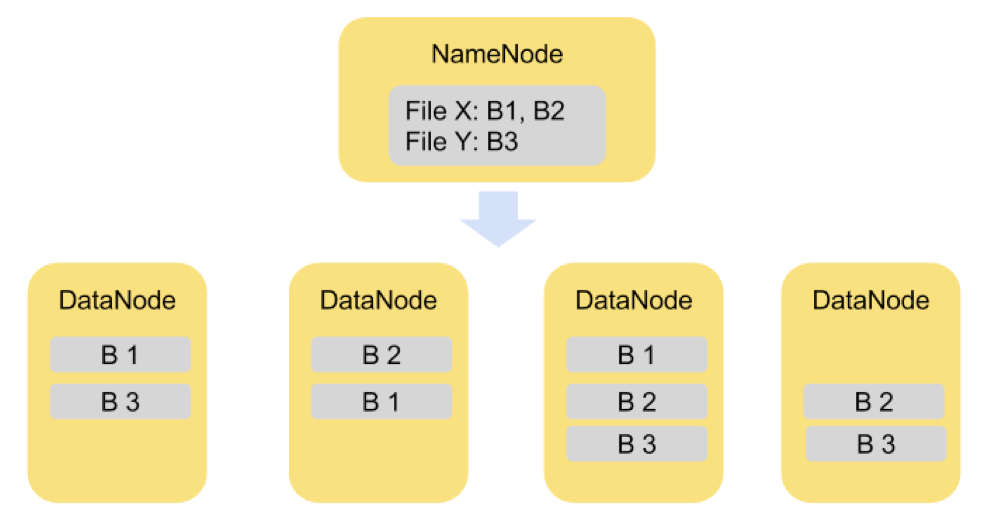
\includegraphics[width=\textwidth]{img/hdfs1}
\end{frame}


% \begin{frame}[fragile,allowframebreaks]
%   \frametitle{Map-Reduce como generalización de consultas}

%   {\bf Ejemplo}: Imagínese un biólogo marino que hace anotaciones de cada
%   animal que ve en el océano, y quiere saber cuántos tiburones ha visto por
%   mes:

%   \begin{lstlisting}[language=SQL]
% SELECT MONTH(observation_timestamp) AS observation_month,
%        sum(num_animals) AS total_animals
% FROM observations
% WHERE family = 'Sharks'
% GROUP BY observation_month;
% \end{lstlisting}

%   \framebreak

% MongoDB con el API de MapReduce:
% \begin{lstlisting}[language=Javascript,basicstyle=\footnotesize\tt]
% db.observations.mapReduce(
%   function map() {
%     var year = this.observationTimestamp.getFullYear();
%     var month = this.observationTimestamp.getMonth() + 1;
%     emit(year + "-" + month, this.numAnimals);
%   },
%   function reduce(key, values) {
%     return Array.sum(values);
%   },
%   {
%     query: { family: "Sharks" },
%     out: "monthlySharkReport"
%   });
% \end{lstlisting}

% \end{frame}

\section{Introducción a NoSQL}

\begin{frame}
  \frametitle{NoSQL}
  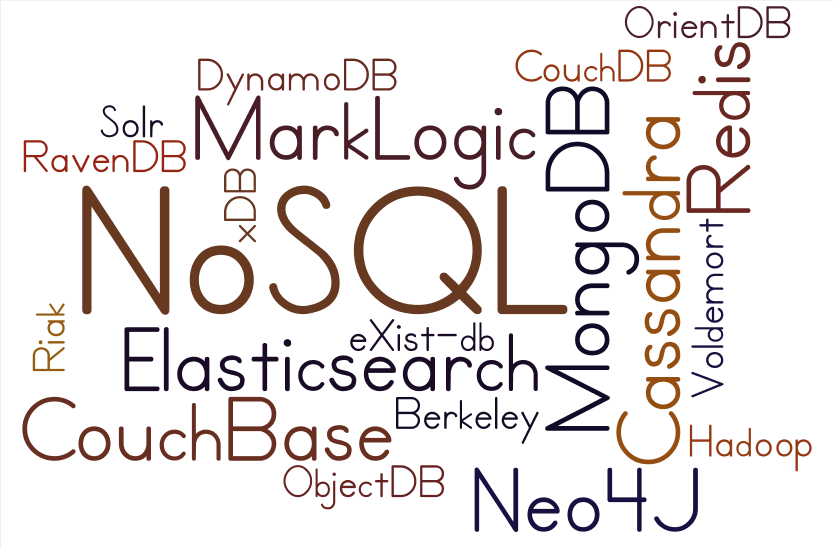
\includegraphics[width=\textwidth]{img/nosql}
\end{frame}

\begin{frame}
  \frametitle{NoSQL}
\begin{itemize}
% \item Sobre los \~{}2010s, se renueva la búsqueda de la escalabilidad, con
%   el abaratamiento del {\em hardware}
% \item Se {\bf diversifican los problemas}, la inclusión del {\bf análisis
%     de todos los datos disponibles por parte de las empresas}
% \begin{itemize}
% \item incluso de algunos que no se había pensado usar, p. ej. {\em
%     clickstreams\/}), {\bf publicidad a la carta}, etc.
% \end{itemize}
\item {\bf NoSQL} \ra{} {\em hashtag\/} llamativo que se
  eligió para una conferencia en~2009 (Johan Oskarsson de Last.fm)
\item Ahora se asocia a cientos de bases de datos diferentes,
  que se han clasificado en varios tipos (las veremos después),
  caracterizadas por {\bf no usar SQL} como modelo de datos
\item {\bf NoSQL} \ra{} {\bfseries\itshape Not Only SQL} (no sólo SQL)
% \item Big Data \ra{} hay una variedad de fuentes de datos ({\bf persistencia
%     polígota})
  \end{itemize}
\end{frame}


\begin{frame}
  \frametitle{Representación relacional de un CV}
\framesubtitle{Kleppmann, 2016. \emph{Designing Data Intensive Applications}}
  \centering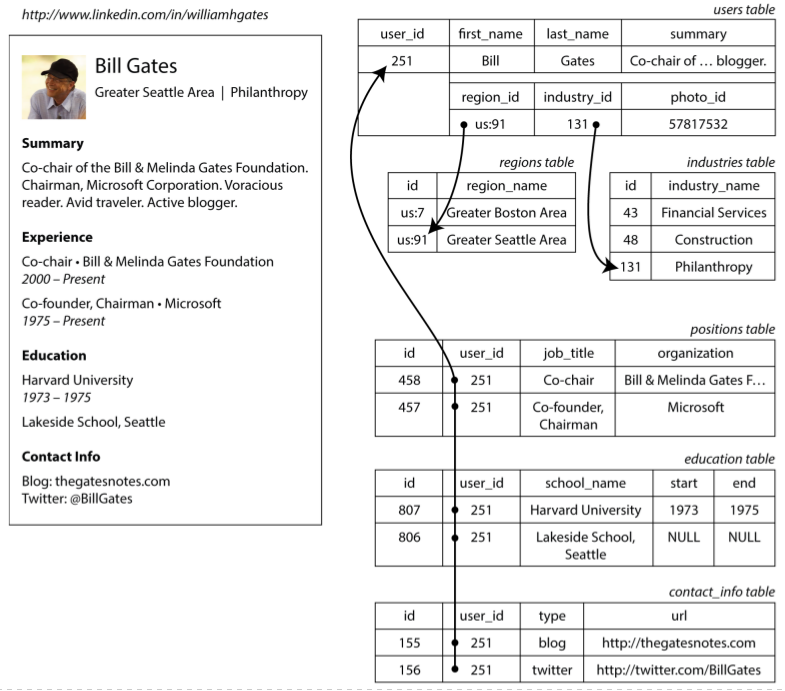
\includegraphics[height=.81\textheight]{img/gates}
\end{frame}

\begin{frame}[plain,fragile]
%  \frametitle{CV como un documento}
\begin{lstlisting}[language=json,basicstyle=\tiny\tt]
{
  "user_id": 251,
  "first_name": "Bill",
  "last_name": "Gates",
  "summary": "Co-chair of the Bill & Melinda Gates... Active blogger.",
  "region_id": "us:91",
  "industry_id": 131,
  "photo_url": "/p/7/000/253/05b/308dd6e.jpg",
  "positions": [
    {
      "job_title": "Co-chair",
      "organization": "Bill & Melinda Gates Foundation"
    },
    {
      "job_title": "Co-founder, Chairman",
      "organization": "Microsoft"
    }
  ],
  "education": [
    {
      "school_name": "Harvard University",
      "start": 1973,
      "end": 1975
    },
    {
      "school_name": "Lakeside School, Seattle",
      "start": null,
      "end": null
    }
  ],
  "contact_info": {
    "blog": "http://thegatesnotes.com",
    "twitter": "http://twitter.com/BillGates"
  }
}
\end{lstlisting}
\end{frame}



% \begin{frame}
%   \frametitle{NoSQL}
% \centering\includegraphics[width=\textwidth]{img/nosqldatabases3}
% \end{frame}

% \begin{frame}
%   \frametitle{NoSQL}
% \centering\includegraphics[width=\textwidth]{img/nosqldatabases}
% \end{frame}

% \begin{frame}[allowframebreaks]
%   \frametitle{NoSQL -- ¿Por qué se plantearon?}
% %En general, el desarrollo de NoSQL ha venido motivado, entre otras, por una
% %serie de circunstancias:
% \begin{enumerate}
% \item {\bf Mayor escalabilidad horizontal}
%   \begin{itemize}
%   \item conjuntos de datos muy muy grandes
%   \item sistemas de alto volumen de escrituras ({\em streaming\/} de
%     eventos, aplicaciones sociales)
%   \end{itemize}
% \item {\bf Demanda de productos de software libre} (crecimiento de las {\em
%     start-ups})
% \item {\bf Consultas especializadas} no eficientes en el modelo relacional
%   (JOINs)
% \item {\bf Expresividad, flexibilidad, dinamismo}. Frustración con {\bf
%     restricciones} del modelo relacional
%   % \ra{} ({\bfseries\itshape schemaless})
% %\item Paradigma {\bf funcional}: {\em Map-Reduce}
% \end{enumerate}

% \framebreak

% \includegraphics[width=\textwidth]{img/data-growth}

% \end{frame}


% \begin{frame}[allowframebreaks]
%  \frametitle{NoSQL: Características}
% \begin{itemize}
% \item No se basan en SQL
% \item Modelos de datos más ricos
% \item Orientadas a la {\bf Escalabilidad}
% \item Generalmente no obligan a definir un esquema \ra{}
%   {\itshape\bfseries Schemaless}
% \item Surgidos de la comunidad para solucionar problemas, y muchas de
%   ellas son {\bf libres/{\itshape open source}}
% \item Diseñadas \ra{} {\bf procesamiento distribuido}
% \item Principios funcionales \ra{} {\bf MapReduce}
% \item Generalmente implementan {\bf consistencia relajada}
% \end{itemize}

% \framebreak

% \begin{block}{Categorías de NoSQL}
%     \begin{itemize}
%     \item Bases de datos Key-Value
%     \item Bases de datos Documentales
%     \item Bases de datos columnares
%     \item Bases de datos de grafos
%     \item Bases de datos de arrays
%     \end{itemize}
% \end{block}
%\end{frame}


% \begin{frame}
%   \frametitle{Evolución desde el modelo relacional}
% \begin{itemize}
% \item El {\bf modelo relacional} $\Rightarrow$ {\bf predominante en los
%   últimos~\~{}30~años}
% \item Tiene sus raíces en el denominado {\em business data processing},
%   procesamiento de transacciones y {\em batch}
% \item Propuesto por Codd en los~70, {\bf de alto nivel}
% \item Actualmente los {\bf sistemas SQL están muy optimizados}:
% \begin{itemize}
% \item el {\bf grado de implantación es mayoritario}
% \item para el 99\% de los problemas (que caben en un ordenador) es
%   eficiente y adecuado
% \end{itemize}
% \end{itemize}
% \end{frame}

% % http://db-engines.com/en/ranking/


% \begin{frame}
%   \frametitle{Adopción de NoSQL}
% Twitter cambiando a Cassandra por~2010\\
% Cassandra desarrollada en Facebook en~2009\\
% \includegraphics[width=\textwidth]{img/twitter-cassandra}
% \end{frame}

% \begin{frame}
%   \frametitle{Adopción NoSQL. Ranking julio 2017}
% \framesubtitle{Fuente: \url{http://db-engines.com/en/ranking/}}
% \vspace*{.1ex}
% \centering\includegraphics[width=.8\textwidth]{img/ranking-bbdd}
% \end{frame}

% \begin{frame}
% \frametitle{Adopción NoSQL.Tendencia julio 2017}
% \framesubtitle{Fuente: \url{http://db-engines.com/en/ranking/}}
% \includegraphics[width=\textwidth]{img/nosql-database-ranking}
% \end{frame}

% \begin{frame}
%   \frametitle{Adopción NoSQL. Análisis}
% \begin{alertblock}{Análisis}
% \begin{itemize}
% \item Dominan los grandes SGBDR
% \item El {\em Open Source} tiene una importancia crucial (MySQL,
%   MongoDB, etc.)
% \item Varias bases de datos NoSQL entre las~10 primeras. Muchas en las~20
%   primeras
% \item La distancia entre los grandes SGBDR y el primer NoSQL (MongoDB) es
%   de~5$\times$
% \item Paradigmas más ``atrevidos'' como el de grafos están entre los~20
%   primeros (Neo4j)
% \end{itemize}
%   \end{alertblock}
% \end{frame}




% \begin{frame}[allowframebreaks]
%   \frametitle{Tecnologías habilitadoras de HBase}
% HBase sobre Hadoop (HDFS y Map-Reduce)
% \begin{itemize}
% \item Una {\bf tabla} está formada por un número de filas, identificadas
%   por una clave
% \item Cada tabla se divide en {\bf regiones} (por rangos de clave ordenada
%   lexicográficamente) ({\bf partición horizontal})
% \item Una instalación de HBase utiliza un conjunto de {\bfseries\itshape
%     Region Servers}: nodos de computación con almacenamiento local (y
%   conectados al clúster HDFS)

% \framebreak

% \item Cada grupo de columnas (llamado {\bfseries\itshape Column~Family\/})
%   se almacena en un {\bf Store} ({\bf partición vertical})
% \item El {\bf Store} tiene una parte en memoria ({\bf MemStore}) y,
%   opcionalmente, un almacenamiento en disco, ({\bf HFile})
% \item Los {\bf HFile} se distribuyen usando HDFS para lograr replicación y
%   tolerancia a fallos
% \end{itemize}
% \end{frame}


% \subsection{Bases de Datos de Grafos}

% \begin{frame}[allowframebreaks]
%   \frametitle{Bases de Datos de Grafos}
% \vspace*{-1ex}
%   \begin{itemize}
%   \item Las bases de datos de grafos llevan el mecanismo {\em muchos a
%       muchos} al extremo
%   \item Datos en los que existen muchas relaciones entre sí y {\bf las
%       relaciones} tienen un significado primordial
% \item Las bases de datos de grafos se basan en la construcción y consulta
%   de un grafo que consta de
%   \begin{itemize}
%   \item {\bf Vértices} también llamados {\em nodos} o {\em entidades}, y
%   \item {\bf Aristas} ({\bfseries\itshape Edges}), también llamados {\em
%       relaciones}
%   \end{itemize}
% \item Los grafos pueden capturar relaciones complejas entre
%   entidades y ofrecen lenguajes de búsqueda, actualización y creación que
%   permiten trabajar con subconjuntos del grafo
% % \item Orígenes en las bases de datos de hechos (con lenguajes de consulta
% %   lógicos (p. ej. {\em Datalog})
% \item Origen en las bases de datos de hechos ({\em Datalog\/})
% \item Ejemplos: FlockDB, Neo4J, OrientDB
% \end{itemize}
% \end{frame}

% \begin{frame}[plain]
% \includegraphics[width=\textwidth]{img/graph}
% \end{frame}

% \begin{frame}[fragile,plain]
% (Nota: Usa la sintaxis PostgreSQL para {\tt json})
% \begin{lstlisting}[language=SQL]
% CREATE TABLE vertices (
%   vertex_id integer PRIMARY KEY,
%   properties json
% );

% CREATE TABLE edges (
%   edge_id integer PRIMARY KEY,
%   tail_vertex integer REFERENCES vertices (vertex_id),
%   head_vertex integer REFERENCES vertices (vertex_id),
%   label text,
%   properties json
% );

% CREATE INDEX edges_tails ON edges (tail_vertex);
% CREATE INDEX edges_heads ON edges (head_vertex);
% \end{lstlisting}
% \end{frame}

\begin{frame}[fragile,allowframebreaks]
  \frametitle{Ejemplo de datos y consulta en Neo4J}
\begin{block}{}
\begin{lstlisting}
CREATE
  (NAmerica:Location {name:'North America', type:'continent'}),
  (USA:Location {name:'United States', type:'country' }),
  (Idaho:Location {name:'Idaho', type:'state' }),
  (Lucy:Person {name:'Lucy' }),
  (Idaho)-[:WITHIN]->(USA)-[:WITHIN]-> (NAmerica),
  (Lucy) -[:BORN_IN]-> (Idaho)
\end{lstlisting}
\end{block}

\framebreak

Y de consulta:
\begin{block}{}
\begin{lstlisting}
MATCH
(person) -[:BORN_IN]-> () -[:WITHIN*0..]-> (us:Location {name:'United States'}),
(person) -[:LIVES_IN]-> () -[:WITHIN*0..]-> (eu:Location {name:'Europe'})
RETURN person.name
\end{lstlisting}
\end{block}

(con esta consulta tan cercana al lenguaje natural, estamos buscando los
emigrantes de EEUU en Europa)

\end{frame}


% \begin{frame}[allowframebreaks]
%   \frametitle{Aplicabilidad de Grafos}
%   \begin{itemize}
%   \item Los grafos, conceptualmente, aparecen en casi cualquier dominio
%   \item Además, su flexibilidad hace que se puedan aplicar de diferentes
%     formas
%   \item Por ejemplo, una relación de {\em follow\/} entre usuarios:

%     \begin{center}
%       \includegraphics[width=.4\textwidth]{img/graph1}
%     \end{center}
%   \end{itemize}

%     \begin{columns}
%       \begin{column}{.5\textwidth}
%         \begin{itemize}
%       \item (nótese cómo {\bf Billy no ha seguido a Ruth}: las relaciones
%         pueden ser unidireccionales o bidireccionales)

%       \item Incluso se puede usar para guardar el conjunto de mensajes
%         que se intercambian:
%       \end{itemize}
%     \end{column}
%       \begin{column}{.5\textwidth}
%         \begin{center}
%           \includegraphics[width=.8\textwidth]{img/graph2}
%         \end{center}
%       \end{column}
%     \end{columns}

% \end{frame}


% \section{Referencias}

% \begin{frame}[fragile,allowframebreaks]
%   \frametitle{Referencias}

% \begin{thebibliography}{Paternostro, 2009}

% \setbeamertemplate{bibliography item}[book]
% \bibitem[Marz, 2015]{Marz2015}
% Nathan Marz, James Warren
% \newblock {\em Big Data: Principles and best
%   practices of scalable realtime data systems}
% \newblock Manning Publications,~2015

% \bibitem[Redmond, 2012]{Redmond2012}
% Eric Redmond, Jim R. Wilson
% \newblock {\em Seven Databases in Seven Weeks: A Guide to Modern Databases
%   and the NoSQL Movement}
% \newblock Pragmatic  Bookshelf,~2012

% \bibitem[Sadalage, 2013]{Sadalage2013}
% Pramod J. Saldage, Martin Fowler
% \newblock {\em NoSQL Distilled. A Brief Guide to the Emerging World of
%   Polyglot Persistence}
% \newblock Addison-Wesley,~2013

% \bibitem[Wilson, 2012]{Wilson2012}
% Jim R. Wilson, Eric Redmond
% \newblock {\em Seven Databases in Seven Weeks}

% \bibitem[Kleppmann, 2016]{Kleppmann2016}
% Kleppmann
% \newblock  \emph{Designing Data Intensive Applications}

% \bibitem[George, 2011]{George2011}
% Lars George
% \newblock {\em HBase, The Definitive Guide}

% \setbeamertemplate{bibliography item}[online]
% \bibitem[ApacheHBaseTeam, 2016]{ApacheHBaseTeam2016}
%   The Apache HBase Team
%   \newblock {\em Apache HBase Reference Guide}
%   \newblock \url{https://hbase.apache.org/book.html}

% \bibitem[HBaseCon, 2012a]{HBaseCon2012a}
%   Ian Varley
% \newblock Vídeo: {\em HBase Schema Design}
% \newblock
% \url{http://www.cloudera.com/content/dam/www/marketing/resources/events/hbase-con/video-hbasecon-2012-hbasecon-2012.png.landing.html}
% \newblock Transparencias:
% \url{http://es.slideshare.net/ivarley/hbase-schema-design-hbasecon-2012}

% \bibitem[George, 2013]{George2013}
%   Lars George
% \newblock {\em HBase Schema Design}
% \newblock \url{https://2013.nosql-matters.org/cgn/wp-content/uploads/2013/05/HBase-Schema-Design-NoSQL-Matters-April-2013.pdf}
% \newblock Otro vídeo: \url{https://vimeo.com/44715954}
% \newblock Sus transparencias: \url{http://2012.berlinbuzzwords.de/sites/2012.berlinbuzzwords.de/files/slides/hbase-lgeorge-bbuzz12.pdf}

% % \bibitem[Khurana, 2013]{khurana2013}
% % Amandeep Khurana, ;login:
% % \newblock {\em Introduction to HBase Schema Design}
% % \newblock \url{http://0b4af6cdc2f0c5998459-c0245c5c937c5dedcca3f1764ecc9b2f.r43.cf2.rackcdn.com/9353-login1210_khurana.pdf}

% % \bibitem[McDonald, 2015]{mcdonald2015}
% %   Carol McDonald
% %   \newblock {\em Guidelines for HBase Schema Design}
% %   \newblock \url{https://www.mapr.com/blog/guidelines-hbase-schema-design}

% \end{thebibliography}
% \end{frame}


\end{document}

%%% Local variables:
%%% mode: LaTeX
%%% TeX-master: t
%%% ispell-local-dictionary: "spanish"
%%% fill-column: 75
%%% TeX-parse-self: t
%%% TeX-auto-save: t
%%% End:
%%% vim: expandtab shiftwidth=2 tabstop=2
